\documentclass[11pt]{scrreprt}


\usepackage{cmap}

\usepackage[utf8]{inputenc}
\usepackage[T1]{fontenc}
\usepackage[english, ngerman]{babel}

\usepackage{microtype}
\usepackage{csquotes}
\usepackage{enumitem}
\usepackage{amsmath}
\usepackage{amsthm}
\usepackage{amsfonts}
\usepackage{mathtools}
\usepackage{xpatch}

\makeatletter
	\xpatchcmd{\proof}{\@addpunct{.}}{\@addpunct{:}}{}{}
	\setlength{\parindent}{0cm}
\makeatother

\newcounter{thm}
\newtheoremstyle{thmstyle}
  {1em} % Space above
  {1.25em} % Space below
  {} % Body font
  {} % Indent amount
  {\bfseries} % Theorem head font
  {.} % Punctuation after theorem head
  {.5em} % Space after theorem head
  {} % Theorem head spec (can be left empty, meaning `normal')
\theoremstyle{thmstyle} 
\numberwithin{thm}{section}

\newtheorem{beispiel}[thm]{Beispiel}
\newtheorem{bemerkung}[thm]{Bemerkung}
\newtheorem{definition}[thm]{Definition}
\newtheorem{korollar}[thm]{Korollar}
\newtheorem{lemma}[thm]{Lemma}
\newtheorem{satz}[thm]{Satz}
\newtheorem{uebung}[thm]{Übung}

\newtheorem*{bemerkung*}{Bemerkung}
\newtheorem*{definition*}{Definition}
\newtheorem*{lemma*}{Lemma}
\newtheorem*{uebung*}{Übung}


\begin{document}


\chapter*{I. Unrestringierte Probleme}
\setcounter{chapter}{1}
\setcounter{section}{1}

\section*{Einführung}

\subsection*{Lösbarkeit}

\setcounter{section}{2}
\setcounter{thm}{2}

\begin{definition}[Lösbarkeit] ~\\
	Das Minimierungsproblem $P$ heißt \textbf{lösbar}, falls ein $\overline{x} \in M$ existiert mit
	$$ \inf_{x \in M} f(x) = f(\overline{x}) $$
\end{definition}

\setcounter{thm}{4}

\begin{satz}
	Das Minimierungsproblem $P$ ist genau dann lösbar, wenn es einen globalen Minimalpunkt besitzt.
\end{satz}

\begin{bemerkung*}
	Es können drei Fälle der Unlösbarkeit auftreten:

	\begin{itemize}
		\item $\inf_{x \in M} f(x) = + \infty$
		\item $\inf_{x \in M} f(x) = - \infty$
		\item Ein endliches Infimum wird nicht angenommen.
	\end{itemize}	
\end{bemerkung*}


\begin{satz}[Satz von Weierstraß] ~\\
	Die Menge $M \subseteq \mathbb{R}^n$ sei nichtleer und kompakt, und die Funktion $f \colon M \rightarrow \mathbb{R}$ sei stetig. Dann besitzt $f$ auf $M$ (mindestens) einen globalen Minimalpunkt und einen globalen Maximalpunkt.
\end{satz}

\setcounter{thm}{7}

\begin{definition}[Untere Niveaumenge]
	Für $X \subseteq \mathbb{R}^n, f \colon X \rightarrow \mathbb{R}$ und $\alpha \in \mathbb{R}$ heißt
	$$ \operatorname{lev}_{\leq}^{\alpha}(f, X) = \big\{ x \in X ~|~ f(x) \leq \alpha \big\} $$
	\textbf{untere Niveaumenge von $f$ auf $X$ zum Niveau $\alpha$}. Im Fall $X = \mathbb{R}^n$ schreiben wir auch kurz
	$$ f_{\leq}^{\alpha} \coloneqq \operatorname{lev}_{\leq}^{\alpha}(f, \mathbb{R}^n) = \big\{ x \in \mathbb{R}^n ~|~ f(x) \leq \alpha \big\} $$
\end{definition}

\setcounter{thm}{9}

\begin{uebung}
	Für eine abgeschlossene Menge $X \subseteq \mathbb{R}^n$ sei die Funktion $f \colon X \rightarrow \mathbb{R}$. Dann ist die Menge $\operatorname{lev}_{\leq}^{\alpha}(f, X)$ für alle $\alpha \in \mathbb{R}$ abgeschlossen.	
\end{uebung}

\begin{uebung}
	Für eine abgeschlossene Menge $X \subseteq \mathbb{R}^n$ und endliche Indexmengen $I$ und $J$ seien die Funktion $g_i \colon X \rightarrow \mathbb{R}, i \in I$, und $h_j \colon X \rightarrow \mathbb{R}, j \in J$, stetig. Dann ist die Menge 
		$$ M = \big\{ x \in X ~|~g_i(x) \leq 0, i \in I, ~ h_j(x) = 0, j \in J \big\} $$
		abgeschlossen.	
\end{uebung}

\begin{definition*}
	Die Menge der globalen Minimalpunkte lautet:
	$$ S = \big\{ \overline{x} \in M ~|~ \forall x \in M: f(x) \geq f(\overline{x}) \big\} $$
\end{definition*}

\begin{lemma}
	Für ein $\alpha \in \mathbb{R}$ sei $\operatorname{lev}_{\leq}^{\alpha}(f, M) \neq \emptyset$. Dann gilt 
	$$ S \subseteq \operatorname{lev}_{\leq}^{\alpha}(f, M). $$
\end{lemma}

\begin{satz}[Verschärfter Satz von Weierstraß]
	Für eine (nicht notwendigerweise beschränkte oder abgeschlossene) Menge $M \subseteq \mathbb{R}^n$ sei $f \colon M \rightarrow \mathbb{R}$ stetig, und mit einem $\alpha \in \mathbb{R}$ sei $\operatorname{lev}_{\leq}^{\alpha}(f, M)$ nichtleer und kompakt. Dann besitzt $f$ auf $M$ (mindestens) einen globalen Minimalpunkt.
\end{satz}

\setcounter{thm}{20}

\begin{definition}[Koerzivität]
	Gegeben seien eine abgeschlossene Menge $X \subseteq \mathbb{R}^n$ und eine Funktion $f \colon \mathbb{R}$ fall für alle Folgen $(x^k) \subseteq X$ mit $\lim_k \| x^k \| = +\infty$ auch
	$$ \lim_k f(x^k) = +\infty $$
	gilt, dann heißt $f$ \textbf{koerziv} auf $X$.
\end{definition}

\setcounter{thm}{23}

\begin{uebung}
		Gegeben sei die quadratische Funktion $q(x) = \frac{1}{2} x^T A x + b^T x$ mit einer symmetrischen $(n, n)$-Matrix $A$ (d.h. es gilt $A = A^T$) und $b \in \mathbb{R}^n$. Die Funktion $q$ ist genau dann koerziv auf $\mathbb{R}^n$, wenn $A$ positiv definit ist (d.h. wenn $d^T A d > 0$ für alle $d\in \mathbb{R}^n \setminus \{ 0 \}$ gilt).
\end{uebung}

\begin{beispiel}
	Auf kompakten Mengen $X$ ist jede Funktion $f$ trivialerweise koerziv.	
\end{beispiel}

\begin{lemma}
	Die Funktion $f \colon X \rightarrow \mathbb{R}$ sei stetig und koerziv auf der (nicht notwendigerweise beschränkten) abgeschlossenen Menge $X \subseteq \mathbb{R}^n$. Dann ist die Menge $\operatorname{lev}_{\leq}^{\alpha}(f, X)$ für jedes Niveau $\alpha \in \mathbb{R}$ kompakt.
\end{lemma}

\begin{korollar}
	Es sei $M$ nichtleer und abgeschlossen, aber nicht notwendigerweise beschränkt. Ferner sei die Funktion $f \colon M \rightarrow \mathbb{R}$ stetig und koerziv auf $M$. Dann besitzt $f$ auf $M$ (mindestens) einen globalen Minimalpunkt.
\end{korollar}

\subsection*{Rechenregeln und Umformungen}

\setcounter{section}{3}
\setcounter{thm}{0}

\begin{uebung}[Skalare Vielfache und Summen]
	Gegeben seien $M \subseteq \mathbb{R}^n$ und $f,g \colon M \rightarrow \mathbb{R}$. Dann gilt
	\begin{enumerate}[label=\alph*\upshape)]
		\item $\forall \alpha \geq 0$, $\beta \in \mathbb{R} \colon \min_{x \in M} \left( \alpha f(x) + \beta \right) = \alpha \left( \min_{x \in M} f(x) \right) + \beta$
		\item $\forall \alpha <0$, $\beta \in \mathbb{R} \colon \min_{x \in M} \left( \alpha f(x) + \beta \right) = \alpha \left( \max_{x \in M} f(x) \right) + \beta$
		\item $\min_{x \in M} \left( f(x) + g(x) \right) \geq \min_{x \in M} f(x) + \min_{x \in M} g(x)$
	\end{enumerate}
\end{uebung}

\begin{uebung}[Separable Zielfunktion auf kartesischem Produkt]
	Es seien $X \subseteq \mathbb{R}^n$, $Y \subseteq \mathbb{R}^m$, $f \colon X \rightarrow \mathbb{R}$ und $g \colon Y \rightarrow \mathbb{R}$. Dann gilt
	$$ \min_{(x,y) \in X \times Y} \left( f(x) + g(y) \right) = \min_{x \in X} f(x) + \min_{y \in Y} g(y) $$	
\end{uebung}

\begin{uebung}[Vertauschung von Minima und Maxima]
	Es seien $X \subseteq \mathbb{R}^n$, $Y \subseteq \mathbb{R}^m$, $M = X \times Y$ und $f \colon M \rightarrow \mathbb{R}$ gegeben. Dann gilt:
	\begin{enumerate}[label=\alph*\upshape)]
		\item $\min_{(x,y) \in M} f(x, y) = \min_{x \in X} \min_{y \in Y} f(x,y) = \min_{y \in Y} \min_{x \in X} f(x, y)$
		\item $\max_{(x,y) \in M} f(x, y) = \max_{x \in X} \max_{y \in Y} f(x,y) = \max_{y \in Y} \max_{x \in X} f(x, y)$
		\item $\min_{x \in X} \max_{y \in Y} f(x, y) \geq \max_{y \in Y} \min_{x \in X} f(x, y)$
	\end{enumerate}
\end{uebung}

\begin{uebung}[Monotone Transformation]
	Zu $M \subseteq \mathbb{R}^n$ und einer Funktion $f \colon M \rightarrow Y$ mit $Y\subseteq \mathbb{R}$ sei $\psi \colon Y \rightarrow \mathbb{R}$ eine streng monoton wachsende Funktion. Dann gilt
	$$ \min_{x \in M} \psi \left( f(x) \right) = \psi \left( \min_{x \in M} f(x) \right), $$
	und die lokalen bzw. globalen Minimalpunkte stimmen überein.
\end{uebung}

\begin{uebung}[Epigraphumformulierung]
	Gegeben seien $M \subseteq \mathbb{R}^n$ und eine Funktion $f \colon M \rightarrow \mathbb{R}$. Dann sind die Probleme
	$$ P \colon \min_{x \in \mathbb{R}^n} f(x) \text{ s.t. } x \in M ~\text{ und } ~ P_{epi} \colon \min_{(x, \alpha) \in \mathbb{R}^n \times \mathbb{R}} \alpha \text{ s.t. } f(x) \leq \alpha, x \in M $$
	äquivalent, d.h. die Minimalwerte stimmen überein und Minimalpunkte entsprechen sich.
\end{uebung}

\begin{definition}[Parallelprojektion]
	Es sei $M \subseteq \mathbb{R}^n \times \mathbb{R}^m$. Dann heißt
	$$ \operatorname{pr}_x M = \big\{ x \in \mathbb{R}^n ~|~\exists y \in \mathbb{R}^m : (x, y) \in M \big\} $$
	\textbf{Parallelprojektion} von $M$ (den \enquote{$x$-Raum}) $\mathbb{R}^n$.
\end{definition}

\begin{uebung}[Projektionsumformulierung]
	Gegeben seien $M \subseteq \mathbb{R}^n \times \mathbb{R}^m$ und eine Funktion $f \colon \mathbb{R}^n \rightarrow \mathbb{R}$, die nicht von den Variablen aus $\mathbb{R}^m$ abhängt. Dann sind die Probleme 
	$$ P \colon \min_{(x, y) \in \mathbb{R}^n \times \mathbb{R}^m} f(x) ~\text{ s.t.} (x, y) \in M ~\text{ und } ~ P_{proj} \colon \min_{x \in \mathbb{R}^n} f(x) \text{ s.t. } x \in \operatorname{pr}_x M $$
	äquivalent, d.h. die Minimalwerte stimmen überein und Minimalpunkte entsprechen sich.
\end{uebung}

\setcounter{chapter}{2}
\setcounter{section}{1}

\newpage

\section*{Optimalitätsbedingungen}

\subsection*{Abstiegsrichtung}

\setcounter{thm}{0}

\begin{definition}[Abstiegsrichtung]
	Es seien $f \colon \mathbb{R}^n \rightarrow \mathbb{r}$ und $\overline{x} \in \mathbb{R}^n$. Ein Vektor $d \in \mathbb{R}^n$ heißt \textbf{Abstiegsrichtung} für $f$ in $\overline{x}$, falls
	$$ \exists \hat{f} > 0 ~\forall t \in (0, \hat{t}) \colon f(\overline{x} + td) < f(\overline{x}). $$
\end{definition}

\begin{uebung}
	Für $f \colon \mathbb{R}^n \rightarrow \mathbb{R}$ sei $\overline{x}$ ein lokaler Minimalpunkt, dann kann keine Abstiegsrichtung für $f$ in $\overline{x}$ existieren.
\end{uebung}

\begin{definition}
	Gegeben seien $f \colon \mathbb{R}^n \rightarrow \mathbb{R}$, ein Punkt $\overline{x} \in \mathbb{R}^n$ und ein Richtungsvektor $d \in \mathbb{R}^n$. Die Funktion
	$$ \varphi_d \colon \mathbb{R}^1 \rightarrow
	 \mathbb{R}^1, ~ t \mapsto f(\overline{x} + td) $$
	 heißt \textbf{eindimensionale Einschränkung} von $f$ auf die durch $\overline{x}$ in Richtung $d$ verlaufende Gerade.
\end{definition}

\begin{bemerkung*}
		Es gilt $\varphi_d(0) = f(\overline{x})$ für jede Richtung $d \in \mathbb{R}^n$. Daher ist $d$ genau dann Abstiegsrichtung für $f$ in $\overline{x}$, wenn
		$$ \exists \hat{t} > 0 ~\forall t \in (0, \hat{t}) \colon \varphi_d(t) < \varphi_d(0) $$
\end{bemerkung*}

\subsection*{Optimalitätsbedingung erster Ordnung}

\begin{definition}
	Eine Funktion $f \colon \mathbb{R}^n \rightarrow \mathbb{R}$ heißt an $\overline{x} \in \mathbb{R}^n$ in eine Richtung $d \in \mathbb{R}^n$ \textbf{einseitig richtungsdifferenzierbar}, wenn der Grenzwert
	$$ f'(\overline{x}, d) \coloneqq \lim_{t \searrow 0} \frac{f(\overline{x} + td) - f(\overline{x})}{t} $$
	existiert. Der Wert $f'(\overline{x}, d)$ heißt dann \textbf{einseitige Richtungsableitung}. Die Funktion $f$ heißt an $\overline{x}$ einseitig richtungsdifferenzierbar, wenn $f$ an $\overline{x}$ in jede Richtung $d \in \mathbb{R}^n$ einseitig richtungsdifferenzierbar ist, und $f$ heißt \textbf{einseitig richtungsdifferenzierbar}, wenn $f$ an jedem $\overline{x} \in \mathbb{R}^n$ einseitig richtungsdifferenzierbar ist.
\end{definition}

\begin{lemma}
	Die Funktion $f \colon \mathbb{R}^n \rightarrow \mathbb{R}$ sei an $\overline{x} \in \mathbb{R}^n$ in Richtung $d \in \mathbb{R}^n$ einseitig richtungsdiffrenzierbar mit $f'(\overline{x}, d) < 0$. Dann ist $d$ Abstiegsrichtung für $f$ in $\overline{x}$.	
\end{lemma}

\begin{lemma}
	Die Funktion $f \colon \mathbb{R}^n \rightarrow \mathbb{R}$ sei an einem lokalen Minimalpunkt $\overline{x} \in \mathbb{R}^n$ einseitig richtungsdifferenzierbar. Dann gilt $f'(\overline{x}, d) \geq 0$ für jede Richtung $d \in \mathbb{R}^n$l
\end{lemma}

\begin{definition}[Abstiegsrichtung erster Ordnung]
	Für eine am Punkt $\overline{x} \in \mathbb{R}^n$ in Richtung $d \in \mathbb{R}^n$ einseitig richtungsdifferenzierbare Funktion $f \colon \mathbb{R}^n \rightarrow \mathbb{R}$ heißt $d$ \textbf{Abstiegsrichtung erster Ordnung}, falls $f'(\overline{x}, d) < 0$ gilt.	
\end{definition}

\begin{definition}[Stationärer Punkt - unrestringierter Fall]
	Die Funktion $f \colon \mathbb{R}^n \rightarrow \mathbb{R}$ sei an $\overline{x} \in \mathbb{R}^n$ einseitig richtungsdifferenzierbar. Dann heißt $\overline{x}$ \textbf{stationärer Punkt} von $f$, falls $f'(\overline{x}, d) \geq 0$ für jede Richtung $d \in \mathbb{R}^n$ gilt.
\end{definition}

\begin{satz}[Kettenregel]
	Es seien $g \colon \mathbb{R}^n \rightarrow \mathbb{R}^m$ differenzierbar an $\overline{x} \in \mathbb{R}^n$ und $f \colon \mathbb{R}^m \rightarrow \mathbb{R}^k$ differenzierbar an $g(\overline{x}) \in \mathbb{R}^m$. Dann ist $f \circ g \colon \mathbb{R}^n \rightarrow \mathbb{R}^k$ differenzierbar an $\overline{x}$ mit
	$$ D( f \circ g )(\overline{x}) = D f( g(\overline{x}) ) \cdot D g(\overline{x}). $$
\end{satz}

\begin{lemma}
	Die Funktion $f \colon \mathbb{R}^n \rightarrow \mathbb{R}$ sei am Punkt $\overline{x} \in \mathbb{R}^n$ differenzierbar, und für die Richtung $d \in \mathbb{R}^n$ gelte $\langle \nabla f(\overline{x}), d \rangle < 0$. Dann ist $d$ Abstiegsrichtung für $f$ in $\overline{x}$.
\end{lemma}

\begin{bemerkung}
	Ein Vektor $d$ ist genau dann eine Abstiegsrichtung erster Ordnung für $f$ in $\overline{x}$, wenn $d$ einen stumpfen Winkel mit dem Gradienten $\nabla f(\overline{x})$ bildet. Wobei das Skalarprodukt genau dann negativ, wenn sie einen stumpfen Winkel miteinander bilden, und analog ist das Skalarprodukt genau für einen spitzen Winkel bildende Vektoren positiv.	
\end{bemerkung}

\begin{uebung}
	Gegeben seien $\overline{x} \in \mathbb{R}^n$, eine endliche Indexmenge $K$ und an $\overline{x}$ differenzierbare Funktionen $f_k \colon \mathbb{R}^n\rightarrow \mathbb{R}$, $k \in K$. Die Funktion $f(x) \coloneqq \max_{k \in K} f_k(x)$ ist an $\overline{x}$ einseitig richtungsdifferenzierbar und dass mit $K_*(\overline{x}) = \{ k \in K ~|~f_k(\overline{x}) = f(\overline{x}) \}$
	$$ f'(\overline{x}, d) = \max_{k \in K_x(\overline{x})} \langle \nabla f_k(\overline{x}), d \rangle $$
	für jede Richtung $d \in \mathbb{R}^n$ gilt.
\end{uebung}

\begin{satz}[Notwendige Optimalitätsbedingung erster Ordnung – Fermat'sche Regel]
	Die Funktion $f \colon \mathbb{R}^n \rightarrow \mathbb{R}$ sei differenzierbar an einem lokalen Minimalpunkt $\overline{x} \in \mathbb{R}$. Dann gilt $\nabla f(\overline{x}) = 0$.
\end{satz}

\begin{definition}[Kritischer Punkt]
	Die Funktion $f \colon \mathbb{R}^n \rightarrow \mathbb{R}$ sei an $\overline{x} \in \mathbb{R}^n$ differenzierbar. Dann heißt $\overline{x}$ kritischer Punkt von $f$, wenn $\nabla f(\overline{x}) = 0$ gilt.
\end{definition}

\begin{uebung}
	Die Funktion $f \colon \mathbb{R}^n \rightarrow \mathbb{R}$ sei differenzierbar an einem Punkt $\overline{x} \in \mathbb{R}^n$. Der Punkt $\overline{x}$ ist genau dann stationärer Punkt von $f$, wenn er kritischer Punkt von $f$ ist.	
\end{uebung}

\setcounter{thm}{16}

\begin{definition}[Sattelpunkt]
	Die Funktion $f \colon \mathbb{R}^n \rightarrow \mathbb{R}$ sei an $\overline{x} \in \mathbb{R}^n$ differenzierbar. Dann heißt $\overline{x}$ \textbf{Sattelpunkt} von $f$, falls $\overline{x}$ zwar kritischer Punkt von $f$, aber weder lokaler Minimal- noch lokaler Maximalpunkt ist.
\end{definition}

\subsection*{Geometrische Eigenschaften von Gradienten}

\begin{center}
	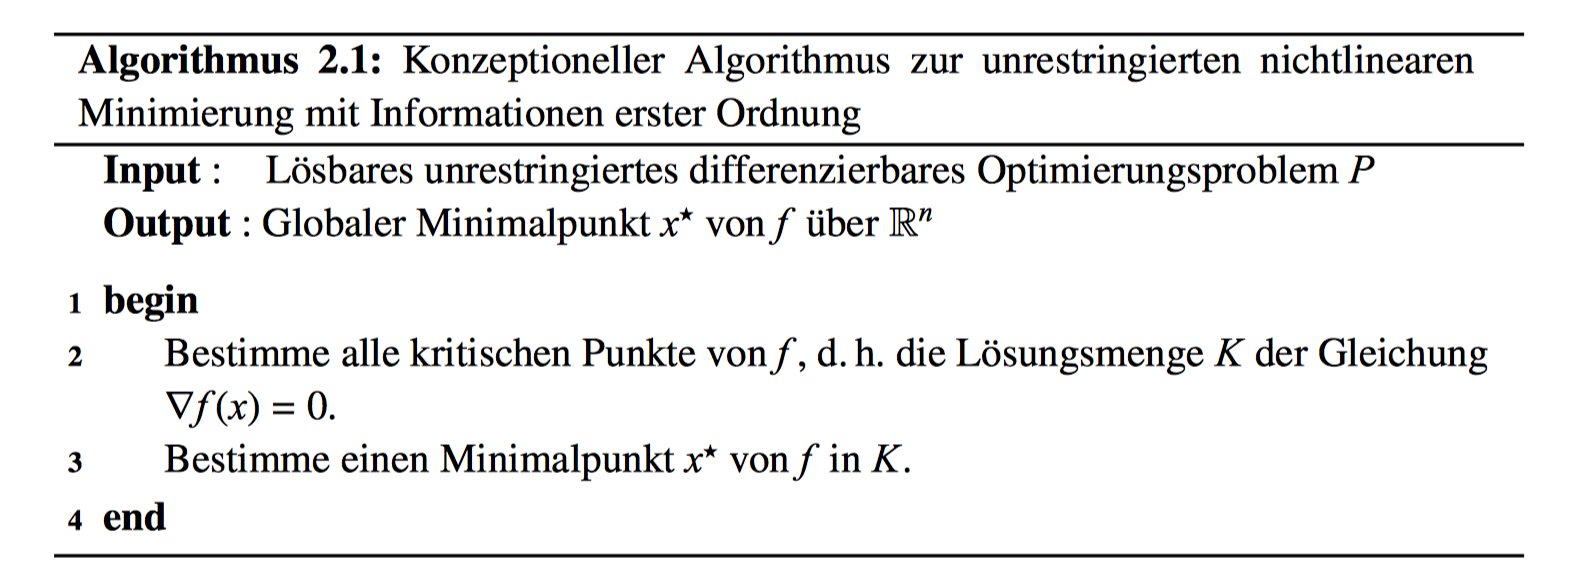
\includegraphics[scale=0.5]{a21}
\end{center}

\begin{center}
	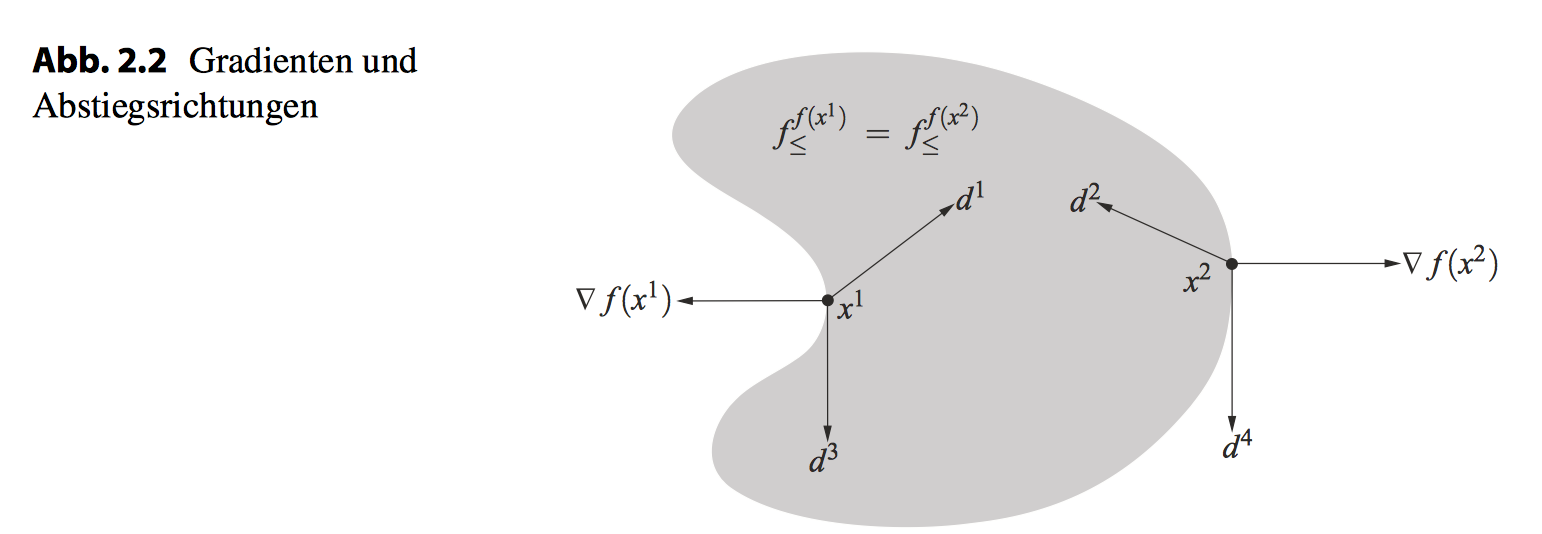
\includegraphics[scale=0.5]{ab22}
\end{center}

\setcounter{thm}{18}

\begin{bemerkung*}
	Man kann zeigen, dass jeder Vektor $d \in \mathbb{R}^n$ mit $\langle \nabla f(\overline{x}), d \rangle > 0$ eine Anstiegsrichtung erster Ordnung ist. Da für einen nichtkritischen Punkt $\overline{x}$ die Gradientenrichtung $d =\nabla f(\overline{x})$ die strikte Ungleichung
	$$ \langle \nabla f(\overline{x}), \nabla f(\overline{x}) \rangle = \{ \nabla f(\overline{x}) \|_2^2 > 0 $$
	erfüllt, ist $d = \nabla f(\overline{x})$ also eine Anstiegsrichtung erster Ordnung für $f$ in $\overline{x}$, und man kann zeigen, dass $\nabla f(\overline{x})$ senkrecht auf dem Rand von $f_{\leq}^{f(\overline{x})}$ steht.
\end{bemerkung*}

\subsection*{Optimalitätsbedingungen zweiter Ordnung}

\begin{bemerkung*}
	Für normierte Richtungen $d$ liefert die Cauchy-Schwarz-Ungleichung 
	$$ - \| \nabla f(\overline{x}) \|_2 = -  \| \nabla f(\overline{x}) \|_2 \cdot \| d \|_2 \leq \langle \nabla f(\overline{x}), d \rangle \leq \| \nabla f(\overline{x}) \|_2 \cdot \| d \|_2 = \| \nabla f(x) \|_2 $$
	und die Unter- und Oberschranken werden genau für linear abhängige $d$ und $\nabla f(\overline{x})$ angenommen. Wegen $\nabla f(\overline{x})$ wird die kleinst- und größtmögliche Steigung daher folgend realisiert
	$$ d_{min} = - \frac{\nabla f(\overline{x})}{\| \nabla f(\overline{x}) \|_2} ~\text{ und }~ d_{max} = \frac{\nabla f(\overline{x})}{\| \nabla f(\overline{x}) \|_2}  $$	
	In der Praxis arbeitet man aber nicht mit der negativen Gradientenrichtung, denn gerade in der Nähe der gesuchten kritischen Punkte - nahe bei null - ist die Division $\frac{\nabla f(\overline{x})}{\| \nabla f(\overline{x}) \|_2}$ numerisch instabil.
\end{bemerkung*}

\begin{satz}[Entwicklungen 1. und 2. Ordnung per univariatem Satz von Taylor] ~\
	\begin{enumerate}[label=\alph*\upshape)]
		\item Es sei $\varphi \colon \mathbb{R} \rightarrow \mathbb{R}$ differenzierbar an $\overline{t}$. Dann gilt für alle $t \in \mathbb{R}$
			$$ \varphi(t) = \varphi(\overline{t}) + \varphi'(\overline{t})(t-\overline{t}) + o(|t - \overline{t}|), $$
			wobei $o(|t-\overline{t}|)$ einen Ausdruck der Form $\omega(t) \cdot |t-\overline{t}|$ mit $\lim_{t \rightarrow \overline{t}} \omega(t) = \omega(\overline{t}) = 0$ bezeichnet.
		\item Es sei $\varphi \colon \mathbb{R} \rightarrow \mathbb{R}$ zweimal differenzierbar an $\overline{t}$. Dann gilt für alle $t \in \mathbb{R}$
			$$\varphi(t) = \varphi(\overline{t}) + \varphi'(\overline{t})(t - \overline{t}) + \frac{1}{2} \varphi''(\overline{t})(t-\overline{t})^2 + o(|t-\overline{t}|^2), $$
			wobei $o(|t-\overline{t}|^2)$ einen Ausdruck der Form $\omega(t) \cdot |t-\overline{t}|^2$ mit $\lim_{t \rightarrow \overline{t}} \omega(t) = \omega(\overline{t}) = 0$ bezeichnet.
	\end{enumerate}
\end{satz}

\begin{lemma}
	Für $f \colon \mathbb{R}^n \rightarrow \mathbb{R}$, einen Punkt $\overline{x} \in \mathbb{R}^n$ und eine Richtung $d \in \mathbb{R}^n$ seien $\varphi'_d(0) = 0$ und $\varphi_d''(0) < 0$. Dann ist $d$ Abstiegsrichtung für $f$ in $\overline{x}$.
\end{lemma}

\begin{lemma}
	Für $f \colon \mathbb{R}^n \rightarrow \mathbb{R}$ sei $\overline{x}$ ein lokaler Minmalpunkt. Dann gilt $\nabla f(\overline{x}) = 0$, und jede Richtung $d \in \mathbb{R}^n$ erfüllt $\varphi_d''(0) \geq 0$.
\end{lemma}

\begin{bemerkung*}
		Es gilt für eine Richtung $d$ gilt, dass $\varphi_d''(0) = d^T D^2 f(\overline{x}) d$
\end{bemerkung*}

\begin{lemma}
	Für $f \colon \mathbb{R}^n \rightarrow \mathbb{R}$, einen Punkt $\overline{x} \in \mathbb{R}^n$ und eine Richtung $d \in \mathbb{R}^n$ seien $\langle \nabla f(\overline{x}), d \rangle = 0$ und $d^T D^2 f(\overline{x}) d < 0$. Dann ist $d$ Abstiegsrichtung für $f$ in $\overline{x}$.
\end{lemma}

\begin{definition}[Abstiegsrichtung zweiter Ordnung]
	Zu $f \colon \mathbb{R}^n \rightarrow \mathbb{R}$ und $\overline{x} \in \mathbb{R}^n$ heißt jeder Richtungsvektor $d \in \mathbb{R}^n$ mit $\langle \nabla f(\overline{x}), d \rangle = 0$ und $d^T D^2 f(\overline{x}) d < 0$ \textbf{Abstiegsrichtung zweiter Ordnung} für $f$ in $\overline{x}$.
\end{definition}

\setcounter{thm}{26}

\begin{satz}[Notwendige Optimalitätsbedingung zweiter Ordnung] ~\
	Die Funktion $f \colon \mathbb{R}^n \rightarrow \mathbb{R}$ sei zweimal differenzierbar an einem lokalen Minimalpunkt $\overline{x} \in \mathbb{R}^n$. Dann gilt $\nabla f(\overline{x}) = 0$ und $D^2 f(\overline{x}) \succeq 0$.	
\end{satz}

\begin{center}
	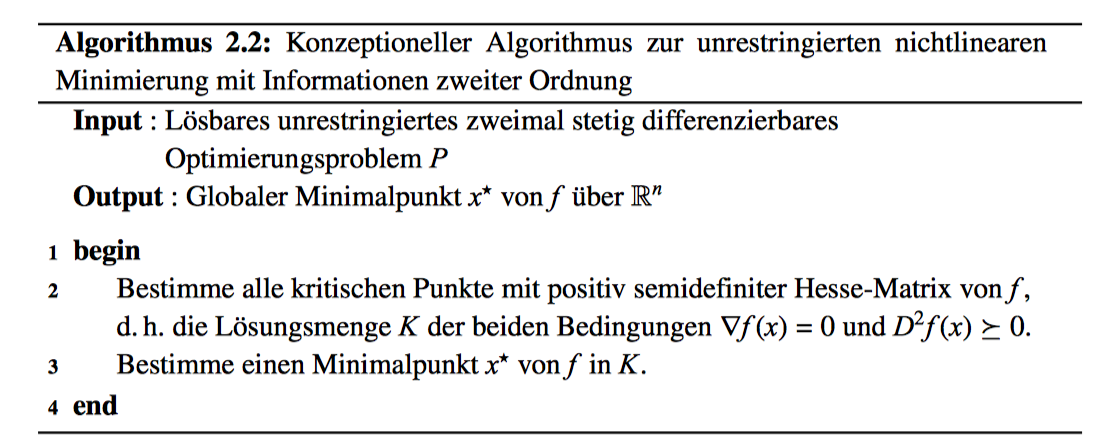
\includegraphics[scale=0.5]{a22}
\end{center}

\setcounter{thm}{29}

\begin{satz}[Entwicklungen 1. und 2. Ordnung per univariatem Satz von Taylor] ~\
	\begin{enumerate}[label=\alph*\upshape)]
		\item Es sei $f \colon \mathbb{R}^n \rightarrow \mathbb{R}$ differenzierbar an $\overline{x}$. Dann gilt für alle $x \in \mathbb{R}^n$
			$$ f(x) = f(\overline{x}) + \langle \nabla f(\overline{x}), x -\overline{x} \rangle + o(\|x - \overline{x}\|), $$
			wobei $o(\|x-\overline{x}\|)$ einen Ausdruck der Form $\omega(x) \cdot \|x-\overline{x}|$ mit $\lim_{x \rightarrow \overline{x}} \omega(x) = \omega(\overline{x}) = 0$ bezeichnet.
		\item Es sei $f \colon \mathbb{R}^n \rightarrow \mathbb{R}$ zweimal differenzierbar an $\overline{x}$. Dann gilt für alle $x \in \mathbb{R}^n$
			$$ f(x) = f(\overline{x}) + \langle f(\overline{x}), x - \overline{x} \rangle + \frac{1}{2} (x-\overline{x})^T D^2 f(\overline{x}) (x-\overline{x}) + o(\|x-\overline{x}\|^2), $$
			wobei $o(\|x-\overline{x}\|^2)$ einen Ausdruck der Form $\omega(x) \cdot \|x-\overline{x}\|^2$ mit $\lim_{x \rightarrow \overline{x}} \omega(x) = \omega(\overline{x}) = 0$ bezeichnet.
	\end{enumerate}
\end{satz}

\begin{definition*} ~\
	\begin{itemize}
		\item $B_{\leq}(\overline{x}, r) = \big\{ x \in \mathbb{R}^n ~|~ \| x - \overline{x} \| \leq r \big\}$
		\item $B_{=}(\overline{x}, r) = \big\{ x \in \mathbb{R}^n ~|~ \| x - \overline{x} \| = r \big\}$
	\end{itemize}	
\end{definition*}

\begin{satz}[Hinreichende Optimalitätsbedingung zweiter Ordnung]
	Die Funktion $f \colon \mathbb{R}^n \rightarrow \mathbb{R}$ sei an $\overline{x} \in \mathbb{R}^n$ zweimal differenzierbar, und es gelte $\nabla f(\overline{x}) = 0$ und $D^2 f(\overline{x}) \succ 0$. Dann ist $\overline{x}$ ein strikter lokaler Minimalpunkt von $f$.
\end{satz}

\setcounter{thm}{34}

\begin{definition}[Nichtdegenerierte kritische und Minimalpunkt] ~\
	Die Funktion $f \colon \mathbb{R}^n \rightarrow \mathbb{R}$ sei an $\overline{x}$ zweimal differenzierbar mit $\nabla f(\overline{x}) = 0$. Dann heißt $\overline{x}$
	\begin{enumerate}[label=\alph*\upshape)]
		\item \textbf{nichtdegenerierter kritischer Punkt}, falls $D^2 f(\overline{x})$ nichtsingulär ist,
		\item \textbf{nichtdegenerierter lokaler Minimalpunkt}, falls $\overline{x}$ lokaler Minimalpunkt und nichtdegenerierter kritischer Punkt ist.
	\end{enumerate}	
\end{definition}

\begin{lemma}
	Der Punkt $\overline{x}$ ist genau dann nichtdegenerierter lokaler Minimalpunkt von $f$, wenn $\nabla f(\overline{x}) = 0$ und $D^2 f(\overline{x}) \succ 0$ gilt.
\end{lemma}

\begin{definition*}
	$\mathcal{F} = \big\{ f \in C^2(\mathbb{R}^n, \mathbb{R}) ~|$ alle kritischen Punkte von $f$ sind nichtdegeneriert $\big\}$	
\end{definition*}

\begin{satz}
	$\mathcal{F}$ ist $C_s^2$-offen und -dicht in $C^2(\mathbb{R}^n, \mathbb{R})$.
\end{satz}

\begin{uebung}
	In einem nichtdegeneriertem Sattelpunkt existiert sowohl eine Ab- als auch eine Anstiegsrichtung zweiter Ordnung.
\end{uebung}

\subsection*{Konvexe Optimierungsprobleme}

\begin{definition}[Konvexe Mengen und Funktionen] ~\
	\begin{enumerate}[label=\alph*\upshape)]
		\item Eine Menge $X \subseteq \mathbb{R}^n$ heißt \textbf{konvex}, falls
			$$ \forall x,y \in X, \lambda \in (0, 1): \quad (1-\lambda) x + \lambda y \in X $$
			gilt (d.h. die Verbindungsstrecke von je zwei beliebigen Punkten in $X$ gehört komplett zu $X$).
		\item Für eine konvexe Menge $X \subseteq \mathbb{R}^n$ heißt eine Funktion $f \colon X \rightarrow \mathbb{R}$ \textbf{konvex} (auf $X$), falls
			$$ \forall x, y \in X, \lambda \in (0, 1): \quad f((1-\lambda) x + \lambda y) \leq (1-\lambda) f(x) + \lambda f(y) $$
			gilt (d.h. der Funktionsgraph von $f$ verläuft unter jeder seiner Sekanten).
	\end{enumerate}
\end{definition}

\begin{bemerkung*}
	Während die Konvexität einer Funktion geometrisch dadurch definiert ist, dass ihr Graph unter jeder ihrer Sekanten verläuft, lässt sich Konvexität einer stetig differenzierbaren Funktion $f$ dadurch charakterisieren, dass ihr Graph über den Graphen jeder ihrer Linearisierungen verläuft.	
\end{bemerkung*}

\begin{center}
	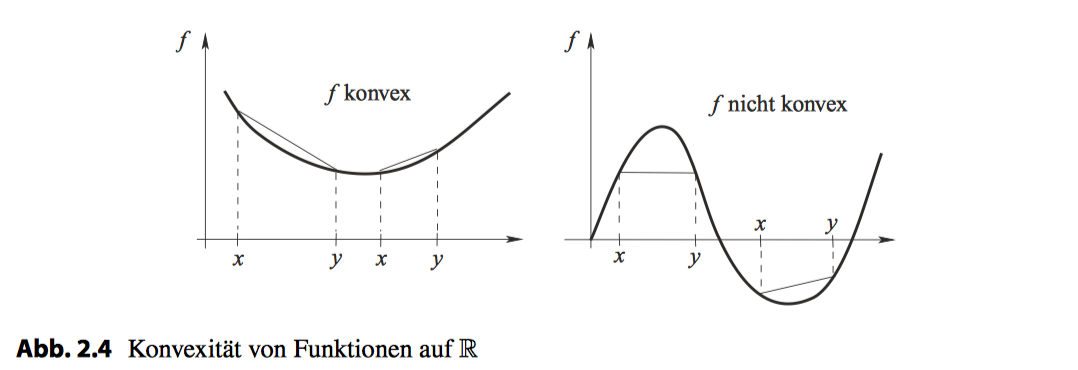
\includegraphics[scale=0.5]{ab24}
\end{center}

\begin{satz}[$C^1$-Charakterisierung von Konvexität]
	Auf einer konvexen Menge $X \subseteq \mathbb{R}^n$ ist eine Funktion $f \in C^1(X, \mathbb{R})$ genau dann konvex, wenn folgendes gilt:
	$$ \forall x,y \in X: \quad f(y) \geq f(x) + \langle \nabla f(x) , y - x \rangle $$	
\end{satz}

\begin{korollar}
	Die Funktion $f \in C^1(\mathbb{R}^n, \mathbb{R})$ sei konvex. Dann sind die kritischen Punkte von $f$ genau die globalen Minimalpunkte von $f$.
\end{korollar}

\begin{satz}[$C^2$-Charakterisierung von Konvexität]
	Eine Funktion $f \in C^2(\mathbb{R}^n, \mathbb{R})$ ist genau dann konvex, wenn folgendes gilt:
	$$ \forall x \in \mathbb{R}^n: \quad D^2 f(x) \succeq 0 $$	
\end{satz}

\begin{uebung}
	Gegeben sei die quadratische Funktion $q(x) = \frac{1}{2} x^T A x + b^T x$ mit $A = A^T \succ 0$ und $b \in \mathbb{R}^n$. Die Funktion $q$ ist eine auf $\mathbb{R}^n$ (gleichmäßige) konvexe Funktion und ihr eindeutiger Minimalpunkt 
	$$ x^* = - A^{-1} b $$
	mit Minimalwert $q(x^*) = - \frac{1}{2}b^T A^{-1} b$.
\end{uebung}

\section*{Numerische Verfahren}

\setcounter{section}{2}
\setcounter{thm}{0}

\subsection{Abstiegsverfahren}
Zunächst betrachten wir Verfahren, die in jedem Iterationsschritt einen Abstieg im Zielfunktionswert erzeugen, für die also

$$ \forall k \in \mathbb{N}_0: \quad f(x^{k+1}) < f(x^k) $$

gilt. Solche Verfahren können nur \enquote{unter sehr unglücklichen Umständen} gegen lokale Maximalpunkte konvergieren und aus geometrischen Überlegungen heraus ist die Konvergenz gegen Sattelpunkte unwahrscheinlich. ~\bigskip

Neben der Stetigkeit der Zielfunktion $f$ werden wir im gesamten Abschn. 2.2 fordern, dass die untere Niveaumenge $f_{\leq}^{f(x^0)}$ zum Startpunkt $x^0 \in \mathbb{R}^n$ beschränkt ist.

\begin{uebung*}
	Als erste algorithmische Idee könnte man versuchen, die Gleichung $\nabla f(x) = 0$ mit dem aus der Numerik bekannten Newton-Verfahren

	$$ x^{k+1} = x^k - \left( D^2 f(x^k) \right)^{-1} \nabla f(x^k), \quad k = 0, 1, 2, \dotsc $$
	
	Vorteil wäre eine hohe Konvergenzgeschwindigkeit, falls $x^0$ nahe genug an einer Lösung liegt. Nachteilig ist, dass $x^0$ nicht in der Nähe einer Lösung zu liegen braucht, dass die Hesse-Matrix $D^2 f ( x^k )$ nicht notwendig invertierbar sein muss und dass das Newton-Verfahren auch gegen lokale Maximalpunkte und Sattelpunkte konvergieren kann.
\end{uebung*}

\begin{center}
	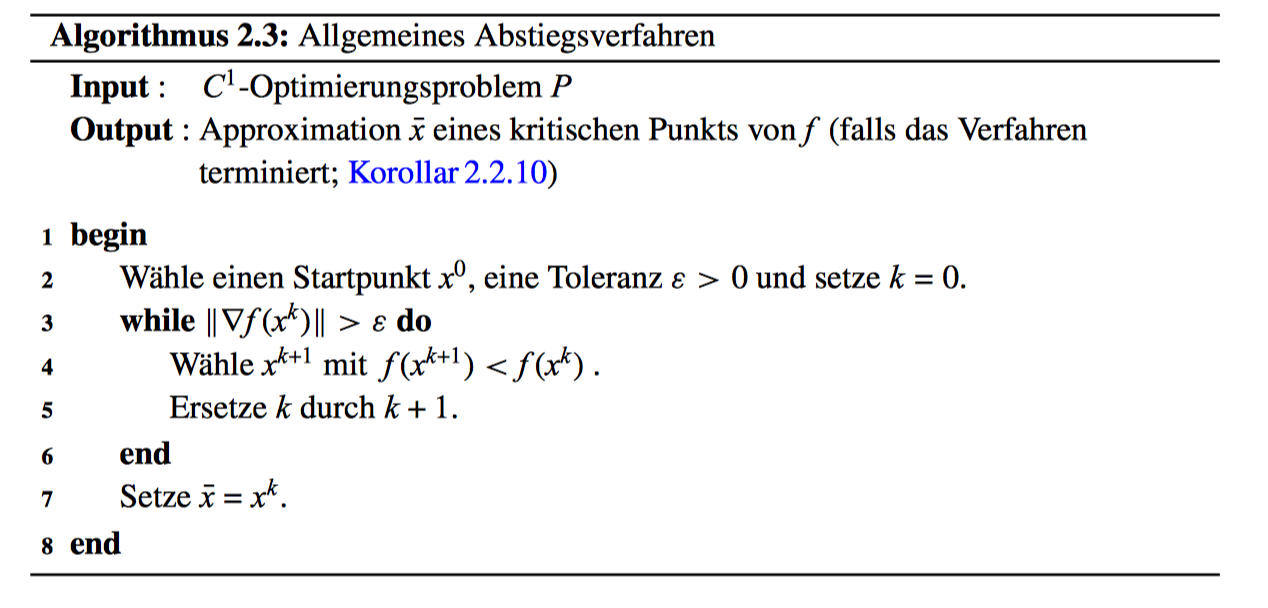
\includegraphics[scale=0.5]{a23}
\end{center}

\setcounter{thm}{2}

\begin{lemma}
	Für beschränktes $f_{\leq}^{f(x^0)}$ bricht die von Algorithmus 2.3 mit $\epsilon = 0$ erzeugte Folge $(x^k)$ entweder nach endlich vielen Schritten mit einem kritischen Punkt ab, oder sie besitzt mindestens einen Häufungspunkt in $f_{\leq}^{f(x^0)}$, und die Folge der Funktionswerte $\left( f(x^k) \right)$ ist konvergent.
\end{lemma}

\setcounter{thm}{4}

\begin{definition}[Effiziente Schrittweiten]
	Es sei $(d^k)$ eine Folge von Abstiegsrichtungen erster Ordnung, und $(t^k)$ erfülle
	$$ \exists c > 0 ~\forall k \in \mathbb{N}: \quad f(x^k+ t^k d^k) - f(x^k) \leq -c \left( \frac{\langle \nabla f(x^k) , d^k \rangle}{\| d^k \|_2} \right)^2 $$
	Dann heißt $(t^k)$ \textbf{effiziente Schrittweitenfolge} für $(d^k)$.
\end{definition}

\begin{satz}
	Die Menge $f_{\leq}^{f(x^0)}$ sei beschränkt, $(d^k)$ sei eine Folge von Abstiegsrichtungen erster Ordnung, und $(t^k)$ sei eine effiziente Schrittweitenfolge. Dann gilt (2.6):
	$$ \lim_{k} \frac{\langle \nabla f(x^k), d^k \rangle}{\| d^k \|_2}	= 0. $$
\end{satz}

\begin{definition}[Gradientenbezogene Suchrichtungen]
	Die Folge von Suchrichtungen $(d^k)$ heißt \textbf{gradientenbezogen}, falls folgendes gilt:
	$$ \exists c > 0 ~\forall k \in \mathbb{N}: \quad \frac{\langle \nabla f(x^k), d^k \rangle}{\| d^k \|_2} \leq - c \cdot \| \nabla f(x^k)\|_2 $$
\end{definition}

\begin{uebung}
	Die Suchrichtungen $d^k = - \nabla f(x^k)$, $k \in \mathbb{N}$ sind gradientenbezogen.
\end{uebung}

\begin{satz}
	Die Menge $f_{\leq}^{f(x^0)}$ sei beschränkt, und in Zeile 4 von Algorithmus 2.3 sei $x^{k+1} = x^k + t^k d^k$ mit einer gradientenbezogenen Suchrichtungsfolge $(d^k)$ und einer effizienten Schrittweitenfolge $(t^k)$ gewählt. Für $\epsilon = 0$ stoppt dann das Verfahren entweder nach endlich vielen Schritten mit einem kritischen Punkt, oder die Folge $(x^k )$ besitzt einen Häufungspunkt, und für jeden solchen Punkt $x^*$ gilt $\nabla f(x^*) = 0$.	
\end{satz}

\begin{korollar}
	Die Menge $f_{\leq}^{f(x^0)}$ sei beschränkt, und in Zeile 4 von Algorithmus 2.3 sei $x^{k+1} = x^k + t^k d^k$ mit einer gradientenbezogenen Suchrichtungsfolge $(d^k)$ und einer effizienten Schrittweitenfolge $(t^k)$ gewählt. Dann terminiert das Verfahren für jedes $\epsilon > 0$ nach endlich vielen Schritten.
\end{korollar}

\subsection*{Schrittweitensteuerung}

\begin{definition*}
	Eine Funktion $F \colon D \rightarrow \mathbb{R}^m$ heißt \textbf{Lipschitz-stetig} auf $D \subseteq \mathbb{R}^n$, falls
	$$ \exists L > 0 ~\forall x, y \in D: \quad \| F(x) - F(y) \|_2 \leq L \cdot \| x - y \|_2 $$
	$C^1$-Funktionen sind auf kompakten Mengen immer Lipschitz-stetig sind, damit ist $\nabla f$ bei beschränkter Menge $f_{\leq}^{f(x^0)}$ zum Beispiel für jede $C^2$-Funktion $f$ Lipschitz-stetig auf $f_{\leq}^{f(x^0)}$.
\end{definition*}

\setcounter{thm}{11}

\begin{bemerkung}
	Bei beschränktem (und daher kompaktem) $f_{\leq}^{f(x^0)}$ ist die Menge $\operatorname{conv}(f_{\leq}^{f(x^0)})$ ebenfalls kompakt, so dass die Forderung der Lipschitz-Stetigkeit von $\nabla f$ auch auf $\operatorname{conv}(f_{\leq}^{f(x^0)})$ eine schwache Voraussetzung ist.	
\end{bemerkung}

\begin{lemma}
	Auf einer konvexen Menge $D \subseteq \mathbb{R}^n$ sei $f$ differenzierbar mit Lipschitz-stetigem Gradienten $\nabla f$ und zugehöriger Lipschitz-Konstante $L > 0$. Dann gilt
	$$ \nabla \overline{x}, x \in D: \quad \left| f(x) - f(\overline{x})- \langle \nabla f(\overline{x}), x - \overline{x} \rangle \right| \leq \frac{L}{2} \| x - \overline{x} \|_2^2 $$
\end{lemma}

\subsubsection*{Exakte Schrittweiten}

Zu $x \in f_{\leq}^{f(x^0)}$ sei eine Abstiegsrichtung erster Ordnung $d$ für $f$ in $x$ gegeben. Wegen $\varphi_d'(0) = \langle \nabla f(x), d \rangle < 0$ gilt $\varphi_d(t) < \varphi_d(0)$ für kleine positive $t$. Für beschränktes $f_{\leq}^{f(x^0)}$ besitzt $\varphi_d$ nach dem Satz von Weierstraß sogar globale Minimalpunkte $t_e> 0$, die exakte Schrittweiten genannt werden. Per Definition der eindimensionalen Einschränkung $\varphi_d$ erfüllen sie
$$ f(x + t_e d) = \min_{t > 0} f(x + td) $$

Eine exakte Schrittweite zu berechnen, um den größtmöglichen Abstieg von $x$ aus entlang d zu erzielen, ist im Allgemeinen sehr aufwendig, so dass wir dieses Konzept meist nur für theoretische Zwecke benutzen werden und später stattdessen zu inexakten Schrittweiten übergehen werden.  Es gilt
	$$ 0 = \varphi_d(t_e) = \langle \nabla f(x + t_ed), d \rangle $$

\begin{uebung}
	Gegeben sei die quadratische Funktion $q(x) = \frac{1}{2} x^T A x + b^T x$ mit $A = A^T \succ 0$ und $b \in \mathbb{R}^n$, die nach Übung 1.2.24 koerziv und nach Übung 2.1.43 konvex ist. Für 
	jedes $x \in \\mathbb{R}^n$ und jede Abstiegsrichtung erster Ordnung $d$ 
	für $q$ in $x$ die exakte Schrittweite eindeutig bestimmt zu
	$$ t_e = - \frac{\langle Ax + b, d \rangle}{d^T A d} $$
\end{uebung}

\begin{satz}
	Die Menge $f_{\leq}^{f(x^0)}$ sei beschränkt, die Funktion $\nabla f$ sei Lipschitz-stetig auf $\operatorname{conv}(f_{\leq}^{f(x^0)})$, und $(d^k)$ sei eine Folge von Abstiegsrichtung erster Ordnung. Dann ist jede Folge von exakten Schrittweiten $(t_e^k)$ effizient.
\end{satz}

\subsubsection*{Konstante Schrittweiten}

Falls die Funktion f keine besondere Struktur aufweist, lohnt sich der Aufwand nicht, in jedem Iterationsschritt eine exakte Schrittweite $t_e^k$ zu berechnen. Daher bnutzt man dann lieber inexakte Schrittweiten, die ebenfalls effizient, aber erheblich leichter zu berechnen sind. ~\bigskip

Eine zunächst naheliegend erscheinende Möglichkeit dafür besteht darin 
 $$ t_c^k = - \frac{\langle \nabla f(x^k), d^k \rangle}{L \cdot \|d^k \|_2^2} $$
Auch diese Schrittweitre ist effizient, genauso wie die exakte. Im speziellen Fall $d^k = -\nabla f (x^k)$ gilt sogar

	$$ t_c^k = \frac{1}{L} $$
	

\subsubsection*{Armijo-Schrittweiten}
	
Eine in modernen Implementierungen von Optimierungsverfahren sehr beliebte inexakte Schrittweitensteuerung geht auf eine Idee von Armijo zurück: Zu $x \in f_{\leq}^{f(x^0)}$ seien $d$ eine Abstiegsrichtung erster Ordnung und $\sigma \in (0,1)$. Dann existiert ein $t > 0$, so dass für alle $t \in (0, \hat{t})$ die Werte $\varphi_d(t)$ unter der \enquote{nach oben gedrehten Tangente} $\varphi_d(0) + t \sigma \varphi_d'(0)$ liegen, so dass also gilt:	
	$$ f(x + td) \leq f(x) + t \sigma \langle \nabla f(x), d \rangle $$
	
	Offensichtlich erfüllt jedes solche $t$££ die Bedingung (2.3):
	$$ \exists c_1 > 0 ~\forall k\in \mathbb{N}: \quad f(x^k + t^k d^k) - f(x^k) \leq c_1 \cdot t^k \langle \nabla f(x^k), d^k \rangle $$
	 mit $c_1 = \sigma$.
	
\begin{center}
	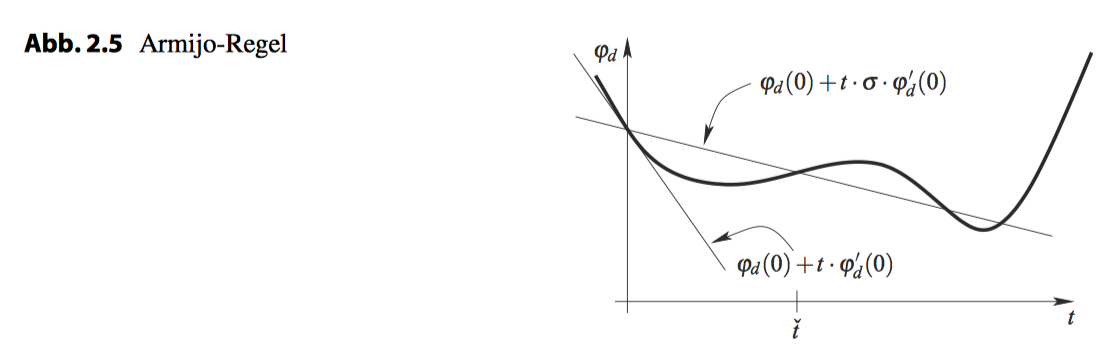
\includegraphics[scale=0.5]{ab25}
\end{center}	

\begin{center}
	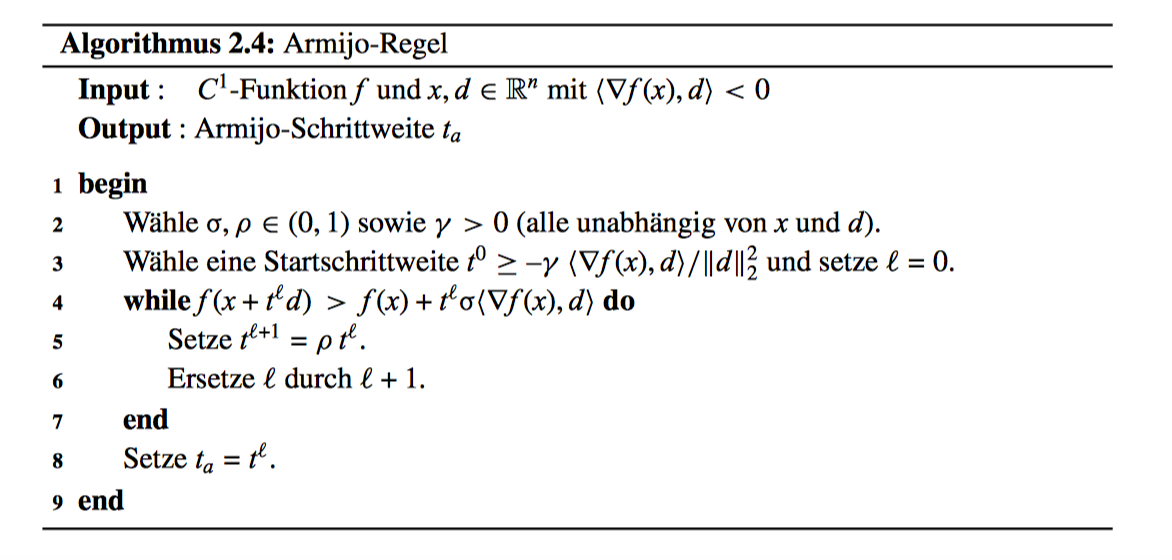
\includegraphics[scale=0.5]{a24}
\end{center}

\begin{satz}
	Die Menge $f_{\leq}^{f(x^0)}$ sei beschränkt, die Funktion $\nabla f$ sei Lipschitz-stetig auf $\operatorname{conv}(f_{\leq}^{f(x^0)})$, und $(d^k)$ sei eine Folge von Abstiegsrichtungen erster Ordnung. Dann ist die Folge der Armijo-Schrittweiten $(t_a^k)$ aus Algorithmus 2.4 (mit unabhängig von $k$ gewählten Parametern $\sigma$, $\rho$ und $\gamma$) wohldefiniert und effizient.
\end{satz}

\begin{uebung}
	Zeigen Sie für die Funktion $f(x) = \frac{1}{2} x^2$, den Startpunkt $x^0 = -3$, die Richtungen $d^k = 2^{-k}$ sowie $\sigma = \frac{1}{2}$, dass der durch die Wahl $t^0 \coloneqq 1$ modifizierte Algorithmus 2.4 nicht zu einer effizienten Schrittweitenfolge führt.
\end{uebung}


Man sollte $t^0$ also so initialisieren, wie in Algorithmus 2.4 angegeben, wobei sich die Wahl $\gamma = 10^{-4}$ bewährt hat. Es ist außerdem nicht schwer zu sehen, dass sich die Armijo-Regel auch für nur einseitig richtungsdifferenzierbare Funktionen einsetzen lässt, indem man das Skalarprodukt $\lambda \nabla f(\overline{x}), d \rangle$ durch $f'(\overline{x}, d)$ ersetzt.

\subsection{Gradientenverfahren}

Aufgrund seiner geometrischen Grundidee ist dies das Verfahren des steilsten Abstiegs.

\begin{center}
	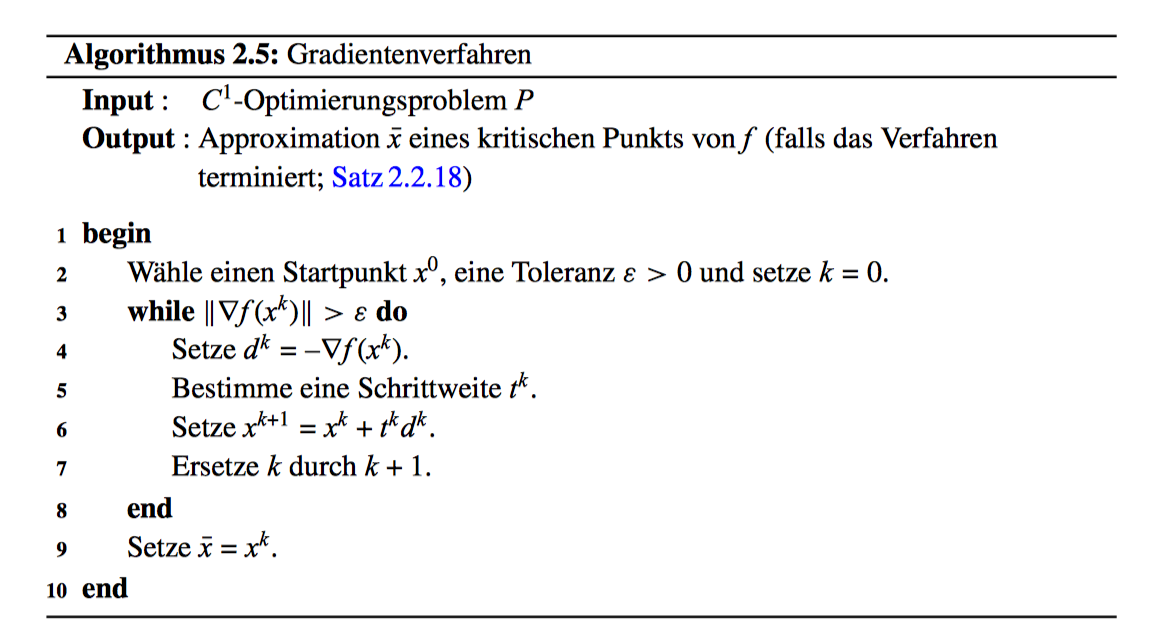
\includegraphics[scale=0.5]{a25}
\end{center}

\begin{satz}
	Die Menge $f_{\leq}^{f(x^0)}$ sei beschränkt, die Funktion $\nabla f$ sei Lipschitz-stetig auf $\operatorname{conv}(f_{\leq}^{f(x^0)})$, und in Zeile 5 seien exakte Schrittweiten $(t_e^k)$ oder Armijo-Schrittweiten $(t_a^k)$ gewählt. Dann terminiert Algorithmus 2.5 für jedes $\epsilon > 0$ nach endlich vielen Schritten. Falls eine Lipschitz-Konstante $L > 0$ zur Lipschitz-Stetigkeit von $\nabla f$ auf $\operatorname{conv}(f_{\leq}^{f(x^0)})$ bekannt ist, dann gilt dieses Ergebnis auch für die dann berechenbaren konstanten Schrittweiten $t_c^k = L^{-1}, k \in \mathbb{N}$.
\end{satz}

\begin{definition*}
	Es ist $\|A\|_2 \coloneqq \max \big\{ \| Ad\|_2 ~|~\| d \|_2 = 1 \big\}$.
\end{definition*}

\begin{uebung}
	Gegeben sei die quadratische Funktion $q(x) = \frac{1}{2} x^T A x + b^T x$ mit $A = A^T$ und $b \in \mathbb{R}^n$. Der Gradient $\nabla q$ ist auf ganz $\mathbb{R}^n$ Lipschitz-stetig mit $L = \| A \|_2$. 
\end{uebung}

\begin{beispiel}
	Nach Übung 2.2.19 erzeugt das Gradientenverfahren eine sogar gegen den globalen Minimalpunkt von $q$ konvergente Folge von Iterierten $(x^k)$, wenn entweder exakte, konstante oder Armijo-Schrittweiten gewählt werden. ~\bigskip
	
	Nach Übung 2.2.14 ist bei jeder Abstiegsrichtung erster Ordnung für $q$ in $x$ die (eindeutige) exakte Schrittweite beim Gradientenverfahren 
	$$ t_e = \frac{\| \nabla q(x) \|_2^2}{D q(x) A \nabla q(x)} $$
\end{beispiel}

Falls die Höhenlinien von $f$ die Form lang gezogener Ellipsen mit einem Minimalpunkt $x^*$ in deren gemeinsamem Zentrum besitzen, dann zeigt $-\nabla f(x^k)$ typischerweise nicht in die Richtung von $x^*$. Die Iterierten springen dadurch entlang einer Zickzacklinie, weshalb man in Anlehnung an die englischsprachige Literatur auch vom Zigzagging-Effekt spricht.

\begin{center}
	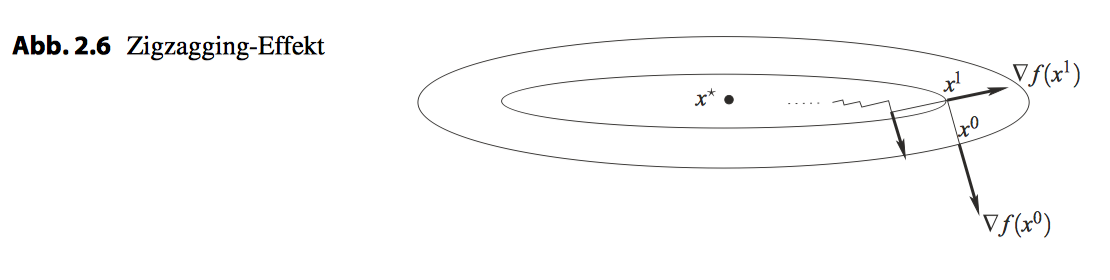
\includegraphics[scale=0.5]{ab26}
\end{center}

\begin{definition}[Konvergenzgeschwindigkeiten]
	Es sei $(x^k)$ eine konvergente Folge mit Grenzpunkt $x^*$. Sie heißt
	\begin{enumerate}[label=\alph*\upshape)]
		\item \textbf{linear konvergent}, falls $\exists 0 < c < 1, ~ k_0 \in \mathbb{N} ~\forall k \geq k_0$: $$ \| x^{k+1} - x^*\| \leq c \cdot \| x^k - x^* \|, $$
		\item \textbf{superlinear konvergent}, falls $\exists c^k \searrow 0, k_0 \in \mathbb{N} ~\forall k \geq k_0$: $$ \| x^{k+1} - x^*\| \leq c^k \cdot \| x^k- x^* \|, $$
		\item \textbf{quadratisch konvergent}, falls $\exists c > 0, k_0 \in \mathbb{N} ~\forall k \geq k_0$: $$ \| x^{k+1} - x^* \| \leq c \cdot \| x^k - x^* \|^2. $$
	\end{enumerate}
\end{definition}

Der folgende Satz zeigt, dass das Gradientenverfahren schon für sehr angenehme Funktionen nur linear konvergente Funktionswerte der Iterierten besitzt, und zwar mit einer Konstante $c$, die sehr nahe bei eins liegen kann. Konkret betrachten wir die konvex-quadratische Funktion $q(x) = \frac{1}{2} x^T A x + b^T x$ mit $A= A^T \succ 0$ sowie $b \in \mathbb{R}^n$ und bezeichnen den größten und den kleinsten Eigenwert der Matrix A mit $\lambda_{max}$ bzw. $\lambda_{min}$ - nach Beispiel 2.2.20 konvergieren dabei die Iterierten des Gradientenverfahrens mit exakten Schrittweiten gegen den globalen Minimalpunkt $x = - A^{-1} b$ von $q$.
    
\begin{lemma}[Kantorowitsch-Ungleichung]
	Es sei $A = A^T \succ 0$ mit maximalem und minimalem Eigenwert $\lambda_{max}$ bzw. $\lambda_{min}$. Dann gilt für jedes $v \in \mathbb{R}^n \setminus \{ 0 \}$
	$$ \frac{v^T A^{-1} v \cdot v^{T} A v}{\| v \|_2^4} \leq \frac{\left(\lambda_{max}+ \lambda_{min} \right)^2}{4 \lambda_{max} \lambda_{min}} $$
\end{lemma}

\begin{satz}
	Auf die konvex-quadratische Funktion $q(x) = \frac{1}{2} x^T A x + b^T x$ mit $A = A^T \succ 0$ und $b \in \mathbb{R}^n$ werde das Gradientenverfahren mit exakten Schrittweiten und $\epsilon = 0$ angewendet. Dann gilt für alle $k \in \mathbb{N}$
	$$ |q(x^{k+1}) - q(x^*)| \leq \left( \frac{\lambda_{max} - \lambda_{min}}{\lambda_{max} + \lambda_{min}} \right)^2 |q(x^k) - q(x^*)|. $$
\end{satz}

Nach Satz 2.2.23 minimiert das Gradientenverfahren (mit exakten Schrittweiten) eine konvex-quadratische Funktion $q(x) = \frac{1}{2}x^T A x + b^T x$ in einem einzigen Schritt, wenn der kleinste und größte Eigenwert $\lambda_{min}$ bzw. $\lambda_{max}$ von $A$ übereinstimmen. Dann stimmen natürlich auch alle Eigenwerte von $A$ miteinander überein, so dass $q$ sphärenförmige Niveaumengen besitzt.

\subsection*{Variable-Metrik-Verfahren}

Im Allgemeinen existiert stets ein rechtwinkliges Koordinatensystem, das zur Lage der ellipsodialen Niveaumengen von $q$ \enquote{passend ausgerichtet} ist, sodass in einem neuen Koordinatensystem die Niveaulinien sphärenförmig sind. ~\bigskip

Für eine nicht notwendigerweise konvex-quadratische Funktion $f \in C^1(\mathbb{R}^n, \mathbb{R})$ beschränkt man sich darauf, approximativ eine Konstruktion wie bei konvex-quadratischen Funktionen zu benutzen:

\setcounter{thm}{26}

\begin{definition}[Gradient bezüglich einer positiv definiten Matrix]
	Für $f \in C^1(\mathbb{R}^n, \mathbb{R})$ und eine $(n, n)$-Matrix $A = A^T \succ 0$ heißt
	$$ \nabla_A f(x) \coloneqq A^{-1} \nabla f(x) $$
	\textbf{Gradient von $f$ bezüglich $A$} an $x$.
\end{definition} 

Die verschiedenen Variable-Metrik-Verfahren unterscheiden sich durch die Wahl der Matrix $A$, mit deren Hilfe die Suchrichtung $- \nabla_A f(x)$ gebildet wird. Für jedes $A = A^T \succ 0$ ist diese Suchrichtung an einem nichtkritischen Punkt $x$ jedenfalls eine Abstiegsrichtung erster Ordnung, denn da mit $A$ auch $A^{-1}$ positiv definit ist, gilt

$$ \langle \nabla f(\overline{x}), - \nabla_A f(\overline{x}) \rangle = - \nabla f(\overline{x})^T A^{-1} \nabla f(\overline{x}) < 0 $$

\begin{uebung}
	Für jedes $A = A^T \succ 0$ ist die Funktion $\langle x, y \rangle_A \coloneqq x^T A y$ ein Skalarprodukt auf $\mathbb{R}^n$.
\end{uebung}

\begin{uebung}
	Für jedes $A = A^T \succ 0$ und für das von $A$ induzierte Skalarprodukt $\langle \cdot, \cdot \rangle_A$ ist die folgende Funktion eine Norm auf $\mathbb{R}^n$:
	$$ \| x \|_A \coloneqq \sqrt{\langle x, x \rangle_{A}} $$
\end{uebung}

\begin{uebung}
	Es gilt unter für die konvex-quadratische Funktion $q(x) = \frac{1}{2} x^T A x + b^T x$ mit $A = A^T \succ 0$, $b \in \mathbb{R}^n$ und mit exakten Schrittweiten:
	$$ \frac{1}{2} \| x - x^* \|_A^2 = q(x) - q(x^*) $$
\end{uebung}

Da die quadrierten Abstände der Iterierten zum Grenzpunkt linear konvergieren, erhält man aus Übung 2.2.30 eine sogar noch langsamere als lineare (nämlich eine sog. sublineare) Konvergenzgeschwindigkeit der Iterierten selbst.

\begin{uebung}
	Gegeben sei die quadratische Funktion $q(x) = \frac{1}{2} x^T A x + b^T x$ mit $A = A^T$ und $b \in \mathbb{R}^n$. Für die exakte Schrittweite des Gradientenverfahrens gilt die Formel 
	$$ t_e = \frac{\| \nabla q(x) \|_2^2}{\| \nabla q(x) \|_A^2} $$
\end{uebung}

\begin{uebung}
	Für das durch $A = A^T \succ 0$ induzierte Skalarprodukt $\langle \cdot, \cdot \rangle_A$ und die induzierte Norm $\| \cdot \|_A$ gilt die Cauchy-Schwarz-Ungleichung:
		$$ \forall x,y \in \mathbb{R}^n: \quad \left| \langle x, y \rangle_A \right| \leq \| x \|_A \cdot \| y \|_A $$
	und die Abschätzung ist scharf.
\end{uebung}

\begin{lemma}
	Es sei $\nabla f(x) \neq 0$. Dann löst der Vektor 
	$$ d = - \frac{- \nabla_A f(x)}{\| \nabla_A f(x) \|_A} $$
	das Problem $\min \langle \nabla f(x), d \rangle$ s.t. $\| d \|_A = 1$, und zwar mit optimalem Wert $- \| \nabla_A f(x) \|_A$.
\end{lemma}

\begin{center}
	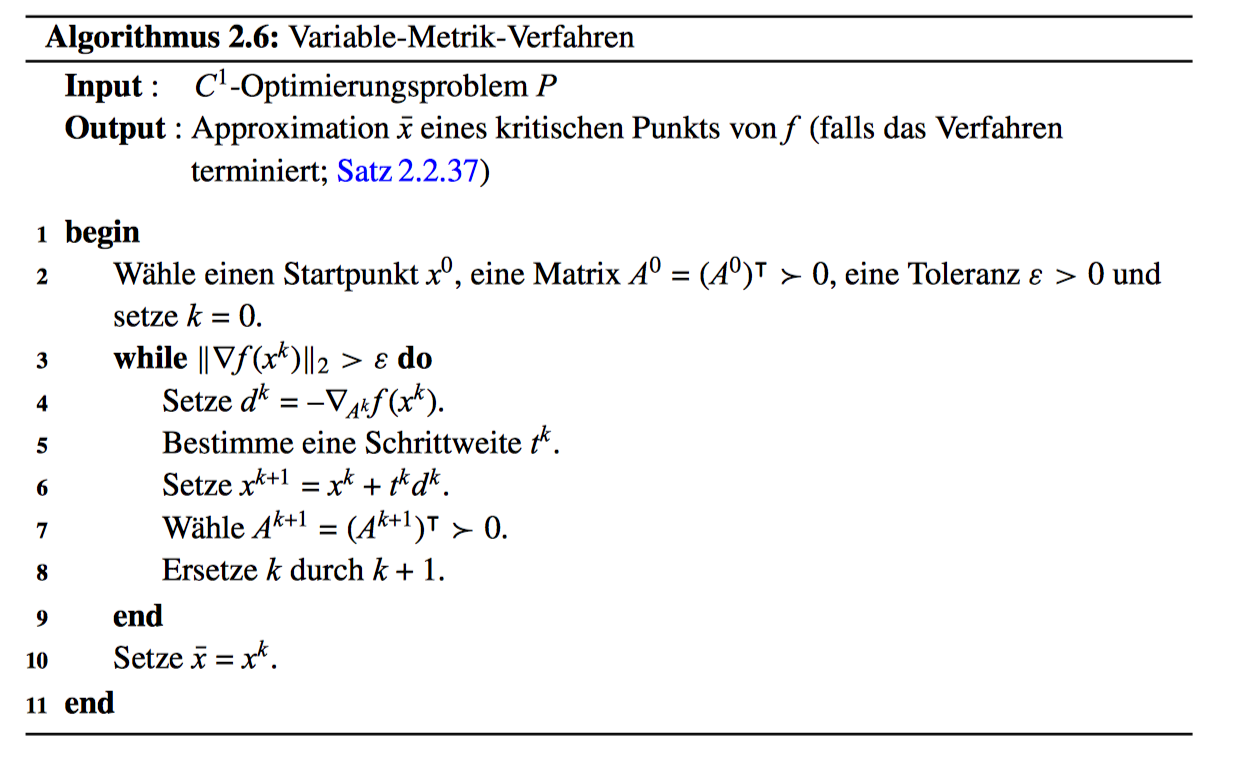
\includegraphics[scale=0.5]{a26}
\end{center}

In Zeile 2 von Algorithmus 2.6 wählt man häufig $A^0 = E$, also als erste Suchrichtung die Gradientenrichtung $d^0 = - \nabla f(x^0)$. In Zeile 3 wäre ein konsistenteres Abbruchkriterium eigentlich 
		$$ \| \nabla_{A^{k}} f(x^k) \|_{A^k} \leq \epsilon, $$
	aber wegen
		$$ \| \nabla_{A^{k}} f(x^k) \|_{A^k} = \sqrt{D f(x^k) (A^k)^{-1} \nabla f(x^k)} = \| \nabla f(x^k) \|_{(A^k)^{-1}} $$
	und der Äquivalenz von $\| \cdot \|_{(A^{k})^{-1}}$ und $\| \cdot \|_2$ (d. h., es gibt Konstanten $c_1, c_2 > 0$, so dass alle $x \in \mathbb{R}^n$ die Abschätzungen $c_1 \| x \|_{(A^{k})^{-1}}\leq \| x \|_2 \leq c_2 \| x \|_{(A^k)^{-1}}$ erfüllen) kann man ebensogut das angegebene und weniger aufwendigere Kriterium testen. In Zeile 4 berechnet man die Suchrichtung $d^k$ numerisch nicht durch die eine Matrixinversion enthaltende Definition $-(A^k)^{-1} \nabla f(x^k)$, sondern weniger aufwendig als Lösung des linearen Gleichungssystems $A^k d = - \nabla f(x^k)$. ~\bigskip

Möchte man die Konvergenz von Variable-Metrik-Verfahren im Sinne von Satz 2.2.9 garantieren, benötigt man neben der Effizienz der Schrittweiten auch die Gradientenbezogenheit der Suchrichtungen. Diese muss man noch fordern.

\begin{definition}[Gleichmäßig positiv definite und beschränkte Matrizen]
	Eine Folge $(A^k)$ symmetrischer $(n,n)$-Matrizen heißt \textbf{gleichmäßig positiv definit} und \textbf{beschränkt}, falls folgendes gilt:
	$$ \exists 0 < c_1 \leq c_2 ~\forall d \in B_{=}(0, 1), ~k \in \mathbb{N}: \quad c_1 \leq d^T A^k d \leq c_2 $$
\end{definition}

\begin{uebung}
	Die Folge $(A^k)$ sei gleichmäßigpositiv definit und beschränkt mit Konstanten $c_1$ und $c_2$. Dann ist die Folge $\left( (A^k)^{-1} \right)$ auch gleichmäßig positiv definit und beschränkt mit Konstanten $\frac{1}{c_2}$ und $\frac{1}{c_1}$. Außerdem ist die Folge $\left( \lambda_{max} \big( (A^k)^{-1} \big) \right)$ der größten Eigenwerte von $\left( (A^k)^{-1} \right)$ durch $\frac{1}{c_1}$ nach oben beschränkt.
\end{uebung}

\begin{satz}
	Die Folge $(A^k)$ sei gleichmäßig positivdefinit und beschränkt. Dann ist die Folge $(d^k)$ mit $d^k = - \left( A^k \right)^{-1} \nabla f(x^k)$, $k \in \mathbb{N}$, gradientenbezogen.
\end{satz}

\begin{satz}
	Die Menge $f_{\leq}^{f(x^0)}$ sei beschränkt, die Funktion $\nabla f$ sei Lipschitz-stetig auf $\operatorname{conv}(f_{\leq}^{f(x^0)})$, die Folge $(A^k)$ sei gleichmäßig positiv definit und beschränkt, und in Zeile 5 seien exakte Schrittweite $(t_e^k)$ oder Armijo-Schrittweiten $(t_a^k)$ gewählt. Dann terminiert Algorithmus 2.6 für jedes $\epsilon > 0$ nach endlich vielen Schritten.
\end{satz}

\begin{bemerkung}[Spektralnorm und Eigenwerte]
		Durch die in Abschnitt 2.2.3 eingeführte Spektralnorm $\|A \|_2 \coloneqq \max \big\{ \| Ad \|_2 ~|~\|d\|_2 = 1 \big\}$ können die Eigenwerte einer Matrix $A$ durch die semidefinite Matrix $A^T A$ berechnet werden. Es ist
		$$ \| A \|_2 = \sqrt{ \lambda_{max}(A^TA)} = \sqrt{ \left( \lambda_{max}(A) \right)^2} = |\lambda_{max}(A) | $$
		Damit ist nach Bemerkung 2.2.24 und Übung 2.2.5 die Länge der längsten Halbachse des Niveau-Ellipsoids
		$$ \frac{1}{\sqrt{\lambda_{min}(A^TA)^{-1})}} = \sqrt{ \lambda_{max}(A^TA)} $$
\end{bemerkung}

\subsection*{Newton-Verfahren mit und ohne Dämpfung}

Wählt man in Algorithmus 2.6 für $f \in C^2(\mathbb{R}^n, \mathbb{R})$ in jedem Schritt $A^k = D^2 f(x^k)$, so erhält man das Newton-Verfahren, sofern die Matrizen $D^2 f (x^k)$ positiv definit sind. ~\bigskip

Ist $x^*$ nichtdegenerierter lokaler Minimalpunkt von $f$, dann gilt aus den bereits am Ende von Abschnitt 2.1.5. aufgeführten Stetigkeitsgründen $D^2 f(x) \succ 0$ für alle $x$ aus einer Umgebung von $x^*$.  Für $x^0$ aus dieser Umgebung  kann man also $A^k = D^2 f (x^k)$ setzen und erhält ein wohldefiniertes Abstiegsverfahren. Ferner sind die Suchrichtungen $d^k = - \left( D^2 f(x^k) \right)^{-1} \nabla f(x^k)$ gradientenbezogen, falls $f$ und $x$ gleichmäßig konvex ist, d. h. falls für eine Umgebung $U$ von $x$ gilt:

	$$ \exists c > 0 ~\forall x \in U, d\in B_{=}(0, 1): \quad c \leq d^T D^2 f(x) d $$
	
Die für diese Folgerung nach Satz 2.2.36 noch erforderliche Beschränktheit der Folge $(D^2 f (x^k ))$ resultiert dabei aus der Stetigkeit von $D^2 f$. Die Nichtdegeneriertheit des lokalen Minimalpunkts $x^*$ gilt bei gleichmäßig konvexem $f$ automatisch. ~\bigskip

Die Dämpfung des Newton-Verfahrens hat den Vorteil, dass der Konvergenzradius (also der mögliche Abstand von $x_0$ zu $x^*$) etwas größer wird. Andererseits ist zunächst nicht klar, ob die Dämpfung nicht auch die lokale Konvergenz verlangsamt. Das ungedämpfte Newton-Verfahren konvergiert unter schwachen Voraussetzungen jedenfalls quadratisch.

\begin{satz}[Quadratische Konvergenz des Newton-Verfahrens]
	Die durch
	$$ x^{k+1} = x^k - \left( D^2 f(x^k) \right)^{-1} \nabla f(x^k) $$
	definierte Folge $(x^k)$ konveriere gegen einen nichtdegenerierten lokalen Minimalpunkt $x^*$, und $D^2 f$ sei Lipschitz-stetig auf einer konvexe Umgebung von $x^*$. Dann konvergiert die Folge $(x^k)$ quadratisch gegen $x^*$.
\end{satz}

\begin{bemerkung}
	Die Voraussetzungen von Satz 2.2.39 lassen sich noch erheblich abschwächen. Erstens gilt die Aussage für jeden nichtdegenerierten kritischen Punkt $x^*$ also nicht nur für lokale Minimalpunkte. Zweitens zeigt Satz 2.2.48, dass die Konvergenz der Folge $(x^k)$ bereits impliziert, dass der Grenzpunt $x^*$ ein nichtdegenerierter kritischer Punkt ist.	
\end{bemerkung}

Die Konvergenzgeschwindigkeit überträgt sich aus Satz 2.2.39 natürlich auf das gedämpfte Newton-Verfahren, falls man mit einem $k_0 \in \mathbb{N}$ für alle $k \geq k_0$ nur $t_k = 1$ wählt. Die folgende Übung gibt eine natürliche Bedingung dafür an.

\begin{uebung}
	Für $f \in C^2(\mathbb{R}^n, \mathbb{R})$ liege $x$ in einer genügend kleinen Umgebung eines nichtdegenerierten lokalen Minimalpunkts, und die Suchrichtung $d$ werde mit dem gedämpften Newton-Verfahren per Armijo-Regel mit $t^0 = 1$ und $\sigma < \frac{1}{2}$ bestimmt. Dann gilt $\langle \nabla f(x), d \rangle < 0$ und dass die Armijo-Regel die Schrittweite $t_a = 1$ wählt.
\end{uebung}

\begin{uebung}
	Das ungedämpfte Newton-Verfahren liefert für die Funktion $q(x) = \frac{1}{2} x^T A x + b^T x$ mit $A = A^T \succ 0$ und $b \in \mathbb{R}^n$ von jedem Startpunkt $x^0 \in \mathbb{R}^n$ nach einem Schritt den globalen Minimalpunkt von $q$.
\end{uebung}

\begin{uebung}
	Für $f \in C^2(\mathbb{R}^n, \mathbb{R})$ sei eine Iterierte $x^k$ mit $D^2 f(x^k) \succ 0$ gegeben. Die vom Newton-Verfahren erzeugte Suchrichtung $d^k$ ist der eindeutige lokale Minimalpunkt der konvex-quadratischen Funktion 
	$$ q(d) = f(x^k) + \langle \nabla f(x^k) , d \rangle + \frac{1}{2} d^T D^2 f(x^k) d $$
\end{uebung}

\begin{bemerkung*}
	Für spezielle Funktionen, wie bei Kleinste-Quadrate-Problemen, also $f(x) = \frac{1}{2} \| r(x) \|_2^2$ mit einer glatten Funktion $r \colon \mathbb{R}^n \rightarrow \mathbb{R}^m$. Es ist
	
	$$ D^2 f(x) = \nabla r(x) D r(x) + \sum_{j=1}^m r_j(x) D^2 r_j(x). $$
	
	Als Modifikation, dem Gauß-Newton-Verfahren, wäre anstatt $A^k = D^2 f (x^k)$ in Zeile 4 $A^k = \nabla r(x^k) Dr(x^k)$ zu wählen. Dass die restlichen Summanden in der Darstellung von eine untergeordnete Rolle spielen, kann zum einen daran liegen, dass für $m \geq n$ überlicherweise ein Punkt $x^*$ mit $r(x^*) = 0$ dass für $m \geq n$ approximiert wird, so dass die Werte $r_j (x^k)$ fast verschwinden, oder zum anderen daran, dass die Krümmung der Funktionen $r_j$ an $x^*$ vernachlässigbar sind, so dass sich die Matrizen $D^2 r_j (x^k)$ in der Nähe der Nullmatrix aufhalten. ~\bigskip
	
	Obwohl zum Aufstellen von $A^k$ im Gauß-Newton-Verfahren also nur Ableitungsinformationen erster Ordnung (die Matrix $Dr(x^k)$) erforderlich sind, lässt sich unter bestimmten Zusatzvoraussetzungen sogar quadratische Konvergenz zeigen. Zusätzlich sind die Suchrichtungen $d^k$ im Gauß-Newton-Verfahren im Gegensatz zum allgemeinen Newton-Verfahren garantiert Abstiegsrichtungen (erster Ordnung), so dass eine Schrittweitensteuerung etwa per Armijo-Regel möglich ist. ~\bigskip
	
	Sollte die Jacobi-Matrix $D r(x^k)$ nicht den vollen Rang besitzen oder zumindest schlecht konditioniert sein, so lässt das Gauß-Newton-Verfahren sich durch die Wahl $A^k = \nabla r(x^k) Dr(x^k) + \sigma^k E$ mit gewissen $\sigma^k > 0$ und der Einheitsmatrix $E$ passender Dimension stabilisieren, was auf das Levenberg-Marquardt-Verfahren führt.
\end{bemerkung*}

\subsection*{Superlineare Konvergenz}

Falls im Newton-Verfahren $x^0$ zu weit von einem nichtdegenerierten Minimalpunkt entfernt liegt, ist $D^2 f (x^k)$ nicht notwendigerweise positiv definit und die Newton-Richtung  entweder nicht definiert oder nicht notwendigerweise eine Abstiegsrichtung. Man versucht daher, das Newton-Verfahren zu globalisieren, d. h. Konvergenz im Sinne von Satz 2.2.9 gegen einen lokalen Minimalpunkt von jedem Startpunkt $x^0 \in \mathbb{R}^n$ aus zu erzwingen. Ein erster Ansatz dazu besteht darin, in Zeile 2 von Algorithmus 2.6 $A^0 = E$ zu wählen sowie in Zeile 7 (ähnlich wie im Levenberg-Marquardt-Verfahren)
		$$ A^{k+1} = D^2 f(x^{k+1}) + \sigma^{k+1} \cdot E $$
	mit einem so großen Skalar $\sigma^{k+1}$, dass $A^{k+1}$ positiv definit ist, und bei hinreichend großen $k$ wieder $\sigma^{k} = 0$ (d. h. das Verfahren startet als Gradientenverfahren und geht nach endlich vielen Schritten in das gedämpfte Newton-Verfahren über). Ein Nachteil des Verfahrens besteht darin, dass die Bestimmung von   $\sigma_k$ sehr aufwendig sein kann: Man halbiert oder verdoppelt $\sigma^{k}$ so lange, bis ein Test auf positive Definitheit von  erfolgreich ist.  ~\bigskip
	
	Im Folgenden werden wir Verfahren kennenlernen, die nicht nach endlich vielen Schritten, sondern nur asymptotisch in das gedämpfte Newton-Verfahren übergehen. Für diese lässt sich immerhin noch superlineare Konvergenz zeigen. Der entsprechende Konvergenzsatz erfordert einige Vorbereitungen.  ~\bigskip
	
	Zunächst besitzt die Folge der Iterierten $(x^k)$ nach Satz 2.2.9 einen Häufungspunkt, und jeder solche Häufungspunkt ist kritisch, sofern die Menge $f_{\leq}^{f(x^0)}$ beschränkt ist und gradientenbezogene Suchrichtungen sowie effiziente Schrittweiten benutzt werden. Die Gradientenbezogenheit der Suchrichtungen wird durch Satz 2.2.36 für gleichmäßig positiv definite und beschränkte $(A^k)$ garantiert. Sei dazu
	
	$$ H^k \coloneqq t^k \left( A^k \right)^{-1}, $$
	
	sodass $x^{k+1} = x^k - H^k \nabla f(x^k)$. Daraus folgt die Definition der superlinearen Konvergenz und diese ist äquivalent zu $\limsup_k \frac{\| x^{k+1} - x^* \|}{\| x^k - x^* \|} = 0$.
	
\setcounter{thm}{45}	
	
\begin{lemma}
	Die Folge $(x^k)$ sei nach obiger Vorschrift gebildet und gegen $x^*$ konvergent. Ferner seien die Folgen $(\| H^k \|_2)$ und $(\| (H^k)^{-1} \|_2)$ beschränkt. Dann gilt
	\begin{enumerate}[label=\alph*\upshape)]
		\item $\nabla f(x^*) = 0$
		\item $\limsup_k \| x^{k+1} - x^* \|_2 / \| x^k - x^*\|_2 \leq \limsup_k \| E - H^k D^2 f(x^*) \|_2$
	\end{enumerate}
\end{lemma}	

\begin{lemma}
	Für zwei $(n,n)$-Matrizen $A$ und $B$ sei $L \coloneqq \| E - AB \|_2 < 1$. Dann gilt
	\begin{enumerate}[label=\alph*\upshape)]
		\item $A$ und $B$ sind nichtsingulär
		\item $\|A\|_2 \leq (1+ L) \cdot \| B^{-1} \|_2$
		\item $\| A^{-1} \| \leq \frac{\| B \|_2}{(1-L)}$
	\end{enumerate}
\end{lemma}
	
\begin{satz}
	Die Folge $(x^k)$ sei nach obiger Vorschrift gebildet und gegen $x^*$ konvergent. Ferner sei $L \coloneqq \limsup_k \| E - H^k D^2 f(x^*) \|_2 < 1$. Dann gelten die folgenden Aussagen:
	
	\begin{enumerate}[label=\alph*\upshape)]
		\item $D^2 f(x^*)$ ist nichtsingulär.
		\item $\nabla f(x^*) = 0$
		\item $(x^k)$ konvergiert mindestens linear gegen $x^*$
		\item Es gilt $L = 0$ genau im Fall von $\lim_k H^k = \left( D^2 f(x^*) \right)^{-1}$, und in diesem Fall konvergiert $(x^k)$ superlinear gegen $x^*$
	\end{enumerate}
\end{satz}	

Nach Satz 2.2.48 sollte Algorithmus 2.6 also asymptotisch in das ungedämpfte Newton-Verfahren übergehen, um superlineare Konvergenz zu garantieren. Wegen

	$$ H^k = t^k \cdot \left( A^k \right)^{-1} $$

sind natürliche Bedingungen dafür $\lim_k t^k = 1$ und $\lim_k A^k = D^2 f(x^*)$. Das zu Beginn dieses Kapitels vorgeschlagene Verfahren erreicht dies mit hohem Aufwand bereits nach endlich vielen Schritten, ist in diesem Sinne also nicht effizient.
	
\subsection*{Quasi-Newton-Verfahren}
	
Ein möglicher Ansatz Matrizen $A^k$ zu finden mit $\lim_k A^k = D^2 f(x^*)$ besteht darin, zunächst das Sekantenverfahren zur Nullstellensuche einer Funktion von $\mathbb{R}$ nach $\mathbb{R}$ zu betrachten. 

\begin{center}
	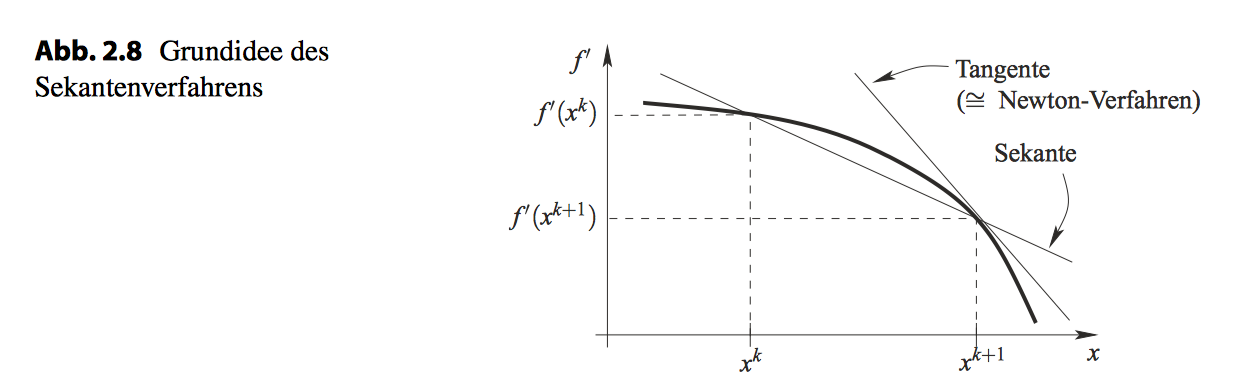
\includegraphics[scale=0.5]{ab28}
\end{center}

Hieraus erhält man für $n \geq 1$ di Gleichung
$$ \nabla f(x^{k+1}) - \nabla f(x^k) = A^{k+1} \cdot \left( x^{k+1} - x^k \right) $$
die als Sekantengleichung oder Quasi-Newton-Bedingung an die $(n, n)$-Matrix $A^{k+1}$ bezeichnet wird. Man zählt leicht nach, dass (2.13) $n$ Gleichungen für die $n^2$ Einträge von $A^{k+1}$ liefert. Selbst wenn man $A^{k+1}$ als symmetrisch voraussetzt, sind noch immer $n(n+1)/2$ Einträge zu bestimmen. Aus diesem Grunde existieren viele Möglichkeiten, verschiedene Quasi-Newton-Verfahren anzugeben. ~\bigskip

Die Grundidee der folgenden Verfahren besteht darin, die Matrix $A^{k+1}$ nicht in jedem Iterationsschritt komplett neu zu berechnen, sondern sie als möglichst einfaches Update der Matrix $A^k$ aus dem vorherigen Schritt aufzufassen. Als erfolgreicher Ansatz hat sich dabei erwiesen, mit $A^0 \succ 0$ zu starten und in Zeile 7 von Algorithmus 2.6 die Matrix $A^{k+1}$ aus $A^k$ durch Addition einer symmetrischen Matrix vom Rang eins oder zwei zu gewinnen:
	$$ A^{k+1} = A^k + \alpha_k (u^k) (u^k)^T + \beta_k (v^k) (v^k)^T $$
	mit Skalaren $\alpha_k, \beta_k \in \mathbb{R}$ und Vektoren $u^k, v^k \in \mathbb{R}^n$, die so gewählt sind, dass $A^{k+1}$ die Sekantengleichung erfüllt. Mit $s^k \coloneqq x^{k+1} - x^k$ und $y^{k} \coloneqq \nabla f(x^{k+1}) - \nabla f(x^k)$ heißt
	$$ A^{k+1} = A + \frac{y y^T}{y^T s} - \frac{As s^T A}{ s^T A s } $$
	BFGS-Update. Da man allerdings in Zeile 4 von Algorithmus 2.6 die Suchrichtung
	$$ d^k = - \left( A^k \right)^{-1} \nabla f(x^k) $$
	wählt, wäre es günstig, die Matrix $(A^k)^{-1}$ explizit angeben zu können.
	
\begin{uebung}[Sherman-Morrison-Woodbury-Formel] ~\
	\begin{enumerate}[label=\alph*\upshape)]
		\item Für eine nichtsinguläre $(n, n)$-Matrix $A$ und Vektoren $b, c \in \mathbb{R}^n$ gelte, dass $A + b c^T$ genau dann nichtsingulär ist, wenn $1 + c^T A^{-1} b$ nicht verschwindet.
		\item Es gilt die Sherman-Morrion-Woodbury-Formel für eine $(n, n)$-Matrix $A$ und Vektoren $b, c \in \mathbb{R}^n$, wobei $A$ und $A + b c^T$ nichtsingulär seien:
			$$ (A + b c^T)^{-1} = A^{-1} - \frac{A^{-1} b c^T A^{-1}}{1 + c^T A^{-1} b} $$ 
	\end{enumerate}
\end{uebung}

Übung 2.2.49 liefert eine Update-Formel für die inversen Matrizen $B \coloneqq A^{-1}$ und $B^+ \coloneqq (A^+)^{-1}$, nämlich
	$$ B_{BFGS}^+ = B + \frac{s s^T}{s^T y} - \frac{By y^T B}{y^T B y} + r r^T $$
	mit $r \coloneqq \sqrt{y^T B y} \cdot \left( \frac{s}{s^T y} - \frac{B y}{y^T B y} \right)$. In Zeile 2 wählt man daher eine Matrix $B^0 \succ 0$ anstelle von $A^0$. In Zeile 4 setzt man
		$$ d^k = -B^k \cdot \nabla f(x^k) $$
		und in Zeile 7 wählt man $B^{k+1} = B_{BFGS}^{k+1}$. Analog kann man auch das DFP-Update definieren, und zwar mit $s$ und $y$ vertauscht
		$$ D_{DFP}^+ = B + \frac{s s^T}{s^T y} - \frac{B y y^T B}{y^T B y} $$
		Dies unterscheidet sich vom BFGS-Update lediglich durch den Term $r r^T$. Die Einführung eines zusätzlichen Parameters $\theta \in \mathbb{R}$ liefert die Updates der Broyden-Familie
		$$ B_{\theta}^+ = B_{DFP}^+ + \theta \cdot r r^T $$
		Offenbar gilt $B_0^+ = B_{DFP}^+$ und $B_1^+ = B_{BFGS}^+$. Außerdem gilt für die Wahl $\theta = \frac{s^T y}{s^T y - y^T B y}$:
		$$ B_{SR1}^+ \coloneqq B_{\theta}^+ = B + \frac{(s- By) (s - By)^T}{(s - By)^T y} $$
		so dass die Update-Matrix nur den Rang 1 besitzt. Man spricht dann vom SR1-Update (SR1 = symmetric rank 1).
		
\begin{uebung}
	Sei $B^k \succ 0$ in einer Iteration eines Quasi-Newton-Verfahrens. Unter der Wahl von exakten Schrittweiten $t^k_e$ gilt die Ungleichung
	$$ (y^k)^T s^k > 0 $$
\end{uebung}	

\begin{lemma}
	Es sei $\theta \geq 0$ beliebig. Dann gilt unter den Bedingungen $B \succ 0$ und $s^T y > 0$ auch $B_{\theta}^+ \succ 0$
\end{lemma}

Zur Division durch die Zahlen $s^T y$ und $y^T B y$ in den Update-Formeln lässt sich also anmerken, dass für mit $B \succ 0$ auch alle iterierten Matrizen $B^k$ positiv definit sind, sofern $(s^k)^T y^k > 0$ positiv ist. Insbesondere gilt dann $y_k \neq 0$ und $(y^k)^T B^k y^k > 0$. Angemerkt sei, dass die Voraussetzung $\theta$ aus Lemma 2.2.51 zwar für den SR1-Update nicht garantiert ist, er in der Praxis aber dennoch häufig gute Ergebnisse liefert. ~\bigskip

Wählt man exakte Schrittweiten $t_e^k$, so hängt nur der Koeffizient des Vektors $r^k$ von $\theta$ ab, und somit ist die Suchrichtung für jedes $\theta \in \mathbb{R}$ identisch. Weil man aber entlang dieser Richtung exakt eindimensional minimiert, liefern alle Verfahren der Broyden-Familie identische Lösungsfolgen $(x^k)$. ~\bigskip

Dieses überraschende Ergebnis wird dadurch relativiert, dass man in der Praxis meist nicht exakt, sondern inexakt eindimensional minimiert, etwa per Armijo-Schrittweitensteuerung mit Backtracking Line Search. Während zum Beispiel das DFPUpdate dazu tendiert, schlecht konditionierte Matrizen $B^k$ zu erzeugen, verhält sich das BFGS-Update für Probleme mittlerer Größe numerisch oft sehr robust. ~\bigskip

Leider lässt sich nicht zeigen, dass die Matrizen $B^k$ stets gegen $(D2f(x^*))^{-1}$ streben, wie es zur Anwendung von Satz 2.2.48 zur superlinearen Konvergenz wünschenswert wäre. Mit einer recht technischen Verallgemeinerung von Satz 2.2.48 lässt sich für $\lim_k t^k = 1$ trotzdem die superlineare Konvergenz der BFGS- und DFP-Verfahren nachweisen, falls $(B^k)^{-1}$ und $D^2 f(x^*)$ wenigstens entlang der Suchrichtungen $d^k$ asymptotisch gleich sind.
		
\subsection*{Konjugierte Richtungen}		
		
Für viele Anwendungsprobleme ist die Anzahl der Variablen so hoch, dass sich zwar Vektoren der Länge $n$ wie $x^k$ und $d^k$ noch gut abspeichern lassen, die Speicherung der $n(n + 1)/2$ Einträge von Matrizen wie $B^k$ aber zu einem Platzproblem führt.	
		
\begin{definition}[Konjugiertheit bezüglich einer positiv definiten Matrix]
	Es sei $A$ eine $(n,n)$-Matrix mit $A = A^T \succ 0$. Zwei Vektoren $v, w \in \mathbb{R}^n$ heißen \textbf{konjugiert bezüglich $A$}, falls $\langle v, w \rangle = 0$ gilt.
\end{definition}	

Im Folgenden betrachten wir das allgemeine Abstiegsverfahren $x^{k+1} = x^k + t_e^k d^k$ mit exakten Schrittweiten $t_e^k$ und Abstiegsrichtungen erster Ordnung $d_k$ für die konvex-quadratische Funktion
	$$ q(x) = \frac{1}{2}x^T A x + b^T x $$
mit $A = A^T \succ 0$ und $b \in \mathbb{R}^n$.

\begin{uebung}
	Für $k \in \mathbb{N}$ seien $d^0, \dotsc, d^k$ paarweise konjugiert bezüglich $A$ und sämtlich ungleich null. Es gilt
	\begin{enumerate}[label=\alph*\upshape)]
		\item Die Vektoren $d^0, \dotsc, d^k$ sind linear unabhängig. insbesondere gilt $k < n$
		\item Für $k = n - 1$ gilt
			$$ A^{-1} = \sum_{l=0}^{n-1} \frac{(d^l)(d^l)^T}{(d^l)^T A (d^l)} $$	
	\end{enumerate}
\end{uebung}	
		
\begin{lemma}
	Für $k\in \mathbb{N}$ seien $d^0, \dotsc, d^k$ paarweise konjugiert bezüglich $A$. Dann gilt
	$$ \forall 0 \leq l \leq k: \quad \langle \nabla q(x^{k+1}), d^l \rangle = 0. $$
\end{lemma}		

\begin{satz}
	Die Vektoren $d^0, \dotsc, d^{n-1}$ seien paarweise konjugiert bezüglich $A$ und sämtlich ungleich null. Dann ist $x^n$ der globale Minimalpunkt von $q$.
\end{satz}
		
Satz 2.2.55 besagt, dass ein Abstiegsverfahren für die konvex-quadratische Funktion $q$ bei exakter Schrittweitensteuerung und paarweise konjugierten Suchrichtungen nach höchstens n Schritten den globalen Minimalpunkt von q findet. Da für ein Abstiegsverfahren wegen $f (x^{k+1}) < f(x^k)$ stets $t_e^k \cdot d^k = x^{k+1} - x^k \neq 0$ gilt, kann insbesondere keiner der Vektoren $d^k$ verschwinden. ~\bigskip

Im nächsten Schritt suchen wir nach Möglichkeiten, konjugierte Suchrichtungen explizit zu erzeugen. Der folgende Satz besagt, dass man konjugierte Richtungen zum Beispiel aus den Quasi-Newton-Verfahren der Broyden-Familie erhält.

\begin{satz}
	Für $\theta \geq 0$ werde Algorithmus 2.6 mit $t^k = t_e^k$ und $B^{k+1} = B^{k+1}_{\theta}$ auf $q() = \frac{1}{2} x^T A x + b^T x$ mit $A = A^T \succ 0$ angewendet, und für ein $k \in \mathbb{N}$ seien die Iterierten $x^0, \dotsc, x^k$ paarweise verschieden. Dann sind die Richtungen $d^0, \dotsc, d^{k-1}$ paarweise konjugiert bezüglich $A$ und sämtlich von null verschieden.
\end{satz}

Bei Wahl exakter Schrittweiten minimieren die Quasi-Newton-Verfahren der Broyden-Familie konvex-quadratische Funktionen also in höchstens $n$ Schritten. Für eine beliebige $C^2$-Funktion $f$ lässt sich das dahingehend interpretieren, dass sie die lokale quadratische Approximation an $f$ in $n$ Schritten minimieren, im Hinblick auf Übung 2.2.43 also einen Schritt des Newton-Verfahrens simulieren. Unter geeigneten Voraussetzungen und mit Neustarts nach jeweils $n$ Schritten konvergieren sie daher \enquote{n-Schritt-quadratisch}.

\subsection*{Konjugierte-Gradienten-Verfahren}

Wir betrachten weiterhin das Abstiegsverfahren $x^{k+1} = x^k + t_e^k d^k$ mit exakten Schrittweiten $t_e^k$ und Abstiegsrichtungen erster Ordnung $d_k$ für die konvex-quadratische Funktion
	$$ q(x) = \frac{1}{2}x^T A x + b^T x $$
mit $A = A^T \succ 0$ und $b \in \mathbb{R}^n$. Gesucht sind Möglichkeiten, konjugierte Suchrichtungen $(d^k)$ zu erzeugen. ~\bigskip

Die Grundidee wird im Folgenden sein, die Suchrichtungen $d^k$ rekursiv zu wählen, nämlich als Kombination des aktuellen negativen Gradienten $-\nabla q(x^k)$ und der letzten Suchrichtung $d^{k-1}$ mit Hilfe eines noch zu bestimmenden \enquote{Gewichts} $\alpha^k  \in \mathbb{R}$ zu
		
		$$ d^k = - \nabla q(x^k) + \alpha_k \cdot d^{k-1}, k = 1,2, \dotsc $$

Zu Beginn dieser Rekursion setzen wir $d^0 = -\nabla q(x^0)$. Das folgende Lemma wird zur Bestimmung der Werte $\alpha_k$ wesentlich sein.

\begin{lemma}
	Es seien $d^0, \dotsc, d^{k-1}$ paarweise konjugiert bezüglich $A$ und $x^1, \dotsc, x^k$ schon generiert mit $x^l \neq x^{l-1}$ für $1 \leq l \leq k$. Dann ist $d^k$ genau dann konjugiert zu einem $d^l$ mit $0 \leq l \leq k-1$, wenn folgendes erfüllt ist
	$$ \langle \nabla q(x^{l+1}) - \nabla q(x^l), d^k \rangle = 0 $$
\end{lemma}

\begin{satz}
	Unter den Voraussetzungen von Lemma 2.2.58 ist die Richtung $d^k = -\nabla q(x^k) + \alpha_k \cdot d^{k-1}$ genau für
	$$ \alpha_k = \frac{\| \nabla q(x^k) \|_2^2}{\| \nabla q(x^{k-1}) \|_2^2} $$
	konjugiert zu den Vektoren $d^0, \dotsc, d^{k-1}$.
\end{satz}

Satz 2.2.58 motiviert den Algorithmus 2.7, da er für $f (x) = q(x) = \frac{1}{2} x^T A x + b^T x$ mit $A = A^T \succ 0$ nach höchstens $n$ Schritten den globalen Minimalpunkt liefert. Man benutzt dieses Verfahren zum Beispiel zur Lösung hochdimensionaler linearer Gleichungssysteme $Ax = b$ durch den Kleinste-Quadrate-Ansatz, also per Minimierung von $\| r(x) \|_2^2$ mit dem Residuum $r(x) = Ax - b$. ~\bigskip

Wegen Rundungsfehlern bricht das Verfahren aber selten tatsächlich nach $n$ Schritten ab, so dass auch seine Konvergenzgeschwindigkeit untersucht wurde. Es stellt sich heraus, dass sie von der Wurzel der Konditionszahl (also dem Quotienten aus größtem und kleinstem Eigenwert) der Matrix $A^T A$ abhängt. Es bietet sich daher an, das Gleichungssystem $Ax = b$ zunächst so äquivalent umzuformen, dass diese Konditionszahl sinkt. Dies ist als Präkonditionierung bekannt.

\begin{center}
	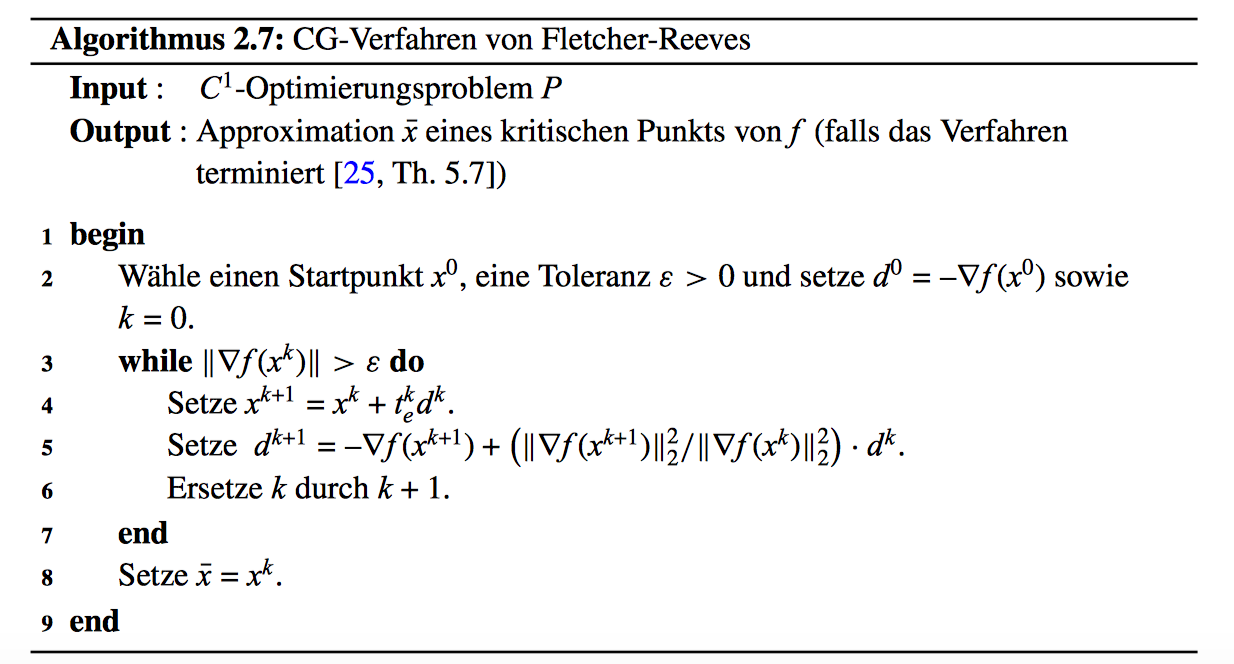
\includegraphics[scale=0.5]{a27}
\end{center}

\begin{bemerkung}
	Der Kleinste-Quadrate-Ansatz per CG-Verfahren zur Lösung linearer Gleichungssysteme $Ax = b$ lässt sich auch auf überbestimmte Gleichungssysteme anwenden, die keine Lösung besitzen.	
\end{bemerkung}

Entscheidend für die Einsetzbarkeit von Algorithmus 2.7 ist, dass für $f = q$ nirgends explizit die Matrix $A$ eingeht, aber trotzdem bezüglich$A$ konjugierte Suchrichtungen erzeugt werden. Man kann das Verfahren also auch für beliebige $C^1$-Funktionen formulieren, wobei die Armijo-Schrittweite für gewöhnlich verwendet wird. Unter geeigneten Voraussetzungen erhält man wieder, dass $n$ CG-Schritte einen Newton-Schritt simulieren, also \enquote{$n$-Schrittquadratische Konvergenz}. 

\subsection*{Trust-Region-Verfahren}

Im Gegensatz zu klassischen Suchrichtungsverfahren wählen Trust-Region-Verfahren erst den Suchradius $t$ und dann die Suchrichtung $d$. Dazu benutzt man in Iteration k des allgemeinen Abstiegsverfahrens aus Algorithmus 2.3 wie folgt ein quadratisches Modell für $f$. ~\bigskip

Nach dem Satz von Taylor (Satz 2.1.30b) gilt für $f \in C^2(\mathbb{R}^n, \mathbb{R})$
$$ f(x^k + d) \approx f(x^k) + \langle \nabla f(x^k) , d \rangle + \frac{1}{2} d^T D^2 f(x^k) d $$
Mit $c^k \coloneqq f(x^k)$, $b^k = \nabla f(x^k)$ und einer symmetrischen Matrix $A^k$ (zum Beispiel, aber nicht notwendigerweise, $A^k = D^2 f(x^k)$) nennt man die Funktion
$$ m^k(d) \coloneqq c^k + \langle b^k, d \rangle + \frac{1}{2} d^T A^k d $$
ein lokales quadratisches Modell für $f$ um $x^k$.  ~\bigskip

Man betrachtet daher $m^k$ nur für $\| d \|_2 \leq t^k$ und bestimmt man einen optimalen Punkt $d^k$ des Trust-Region-Hilfsproblems
$$ TR^k: \quad \min_{d \in \mathbb{R}^n} m^k(d) \text{ s.t. } \| d \|_2 \leq t^k $$
Der folgende Quotient misst dabei die Güte der Approximation
$$ r^k \coloneqq \frac{f(x^k) - f(x^k + d^k)}{m^k(0)- m^k(d^k)} $$

\begin{itemize}
	\item Ein Wert $r^k < 0$ impliziert daher $f (x^k + d^k) > f (x^k)$, d. h., $x^{k+1} = x^k + d^k$ würde einen Anstieg im Zielfunktionswert liefern. Folglich ist die Trust Region zu groß, und ihr Radius $t^k$ muss verkleinert werden.
	\item Liegt andererseits $r^k$ nahe bei eins, dann beschreibt das lokale Modell die Funktion $f$ sehr gut; man setzt $x^{k+1} = x^k + d^k$ und vergrößert in der nächsten Iteration probeweise den Trust-Region-Radius $t^k$.
	\item Insbesondere für $r^k \geq \frac{1}{4}$ wird $t^k$ dort nicht verkleinert, und der Schritt wird angenommen, für $r^k < 0$ wird $t^k$ verkleinert, und der Schritt wird abgelehnt, und für $r^k \in [0, \frac{1}{4})$ wird $t^k$ verkleinert, und der Schritt wird dann abgelehnt, wenn $r^k \leq \eta$ gilt.
\end{itemize}

Ein entscheidender Vorteil von Trust-Region-Verfahren gegenüber Variable-Metrik-Verfahren besteht allerdings darin, dass die Matrizen $A^k$ nicht positiv definit zu sein brauchen. Insbesondere für $A^k \equiv 0$ erhält man als \enquote{Trust-Region-Gradientenverfahren} lediglich ein übliches Gradientenverfahren mit einer speziellen Schrittweitensteuerung. Von einem solchen Verfahren ist wegen Satz 2.2.23 keine schnelle Konvergenz zu erwarten. ~\bigskip

 Allerdings auch hier eine inexakte Lösung von $TR^k$, um globale Konvergenz zu gewährleisten. Eine Möglichkeit dafür besteht darin, die zulässige Menge von TR k stark zu verkleinern und beispielsweise nur nichtnegative Vielfache der beim Verfahren gefundenen Suchrichtung zuzulassen:
$$ TR_C^k: \quad \min_{s \in \mathbb{R}} m^k \left( - \frac{s \cdot t^k}{\| \nabla f(x^k) \|_2} \cdot \nabla f(x^k) \right) \text{ s.t. } 0 \leq s \leq 1 $$
Die Lösung zu diesem Problem ergibt sich $d_C^k \coloneqq - \frac{s^k t^k}{\| \nabla f(x^k) \|_2} \nabla f(x^k)$ mit
$$ s^k \coloneqq \begin{cases} 1, & \text{ falls } Df(x^k) A^k \nabla f(x^k)\leq 0 \\ \min \left\{ \frac{\| \nabla f(^k) \|_2^3}{t^k Df(x^k) A^k \nabla f(x^k)}, 1 \right\}, & \text{ sonst} \end{cases} $$

\begin{center}
	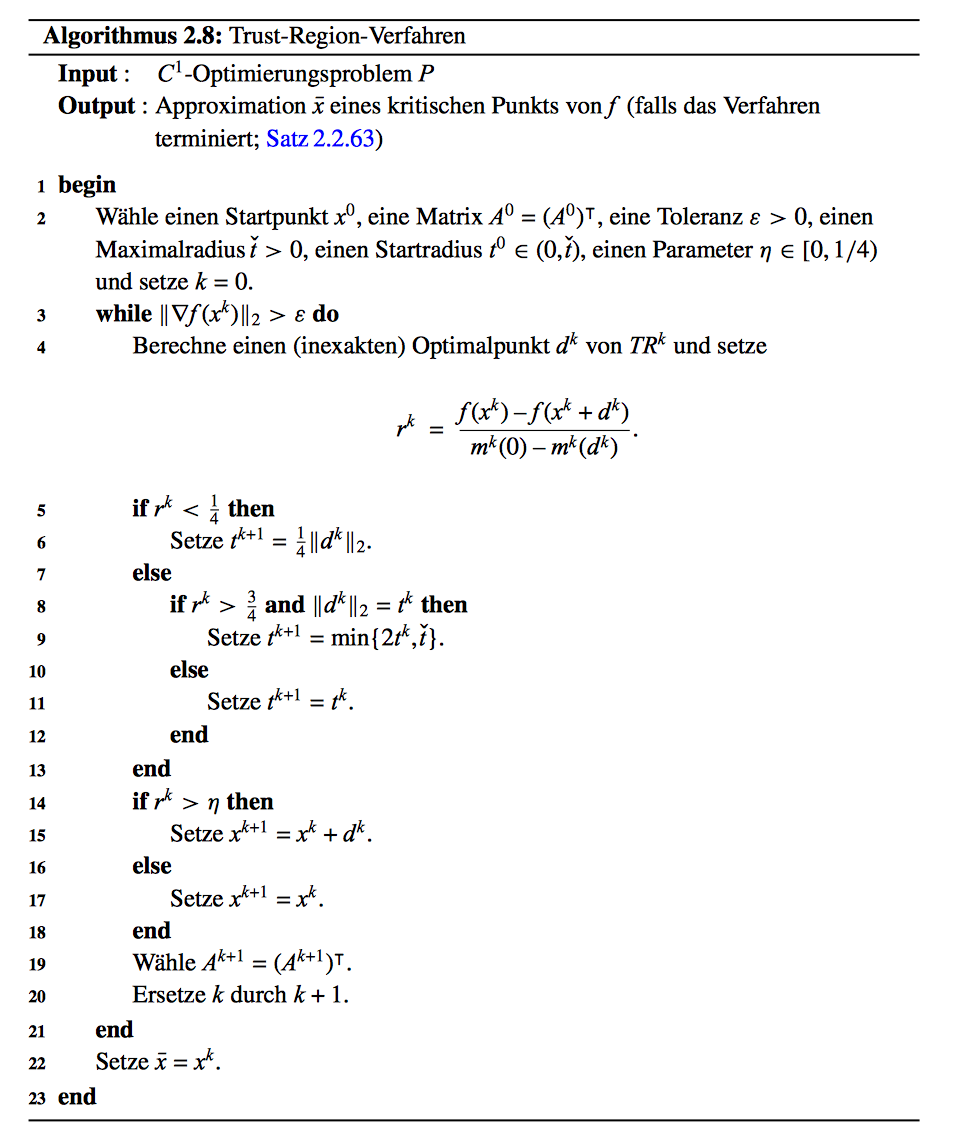
\includegraphics[scale=0.75]{a28}
\end{center}

\begin{definition}[Cauchy-Punkt]
	Der Punkt $x_C^{k+1}	 = x^k + d^k_C$ heißt \textbf{Cauchy-Punkt} zu $x^k$ und $t^k$.
\end{definition}

\begin{uebung}
	Der Vektor $d^k = d_C^k$ erfüllt die folgende Ungleichung mit $c = 0.5$
	\begin{equation}
		m^k(0) - m^k(d^k) \geq c \cdot \| \nabla f(x^k) \|_2 \cdot \min \left\{ t^k, \frac{\| \nabla f(x^k) \|_2}{\| A^k \|_2} \right\}  \tag*{(2.24)}
	\end{equation}
	$$ $$
\end{uebung}

\begin{bemerkung} 
	Die exakte Lösung $d_e^k$ von $TR^k$ erfüllt wegen der Zulässigkeit von $d_C^k$ für $TR^k$ die Ungleichung $m^k (d_e^k) \leq m^k (d_C^k)$ und damit nach Übung 2.2.61 ebenfalls (2.24) mit $c = 0.5$.	
\end{bemerkung}

\begin{satz}
	Die Menge $f_{\leq}^{f(x^0)}$ sei beschränkt, die Funktion $\nabla f$ sei Lipschitz-stetig auf $\operatorname{conv}(f_{\leq}^{f(x^0)})$, die Folge $(\|A^k\|_2)$ sei beschränkt, und die Folge $(d^k)$ der inexakten Lösungen von $TR^k$ erfülle (2.24) mit $c > 0$. Dann gilt in Algorithmus 2.8:
	\begin{enumerate}[label=\alph*\upshape)]
		\item Für $\eta = 0$ ist $\liminf_k \| \nabla f(x^k) \|_2 = 0$ (d.h. $(x^k)$ besitzt einen Häufungspunkt $x^*$ mit $\nabla f(x^*) = 0$).
		\item Für $\eta \in (0, 1)$ ist $\lim_k  \nabla f(x^k) = 0$ (d.h. alle Häufungspunkte von $(x^k)$ sind kritisch).
	\end{enumerate}
\end{satz}

Nach Übung 2.2.61, Bemerkung 2.2.62 und Satz 2.2.63 liefern sowohl die inexakten Lösungen $d_C^k$ als auch die exakten Lösungen $d_e^k$ von $TR^k$ globale Konvergenz. Während die exakte Lösung $d_e^k$ wie erwähnt schwer berechenbar sein kann, ist das Ausweichen auf die inexakte Lösung $d_C^k$ selten ratsam, da die Matrix $A^k$ lediglich die Länge von $d_C^k$ beeinflusst und man so im Wesentlichen nach wie vor das Gradientenverfahren erhält.

\subsubsection*{Dogleg-Methode}

Sei $A$ positiv definit und $d_A \coloneqq - A^{-1} \nabla f(x)$. Die Dogleg-Methode approximiert diese Kurve durch einen Polygonzug von $x$ nach $x+d_A$ mit zwei Segmenten, wobei als Zwischenpunkt $x+d_G$ mit dem exakten Minimalpunkt $d_G$ von $m$ entlang $-\nabla f(x)$ gewählt wird, den man zu
$$ d_G = - \frac{\| \nabla f(x) \|_2^2}{D f(x) A \nabla f(x)} \nabla f(x) $$
berechnet. Formal lautet der Polygonzug damit $\{ x + \hat{d}(s) ~|~ s \in [0, 2] \}$ mit
$$ \hat{d}(s) = \begin{cases}
	s \cdot d_G, & 0 \leq s \leq 1 \\ d_G + (s-1) (d_A - d_G), & 1 \leq s \leq 2
\end{cases} $$

\begin{center}
	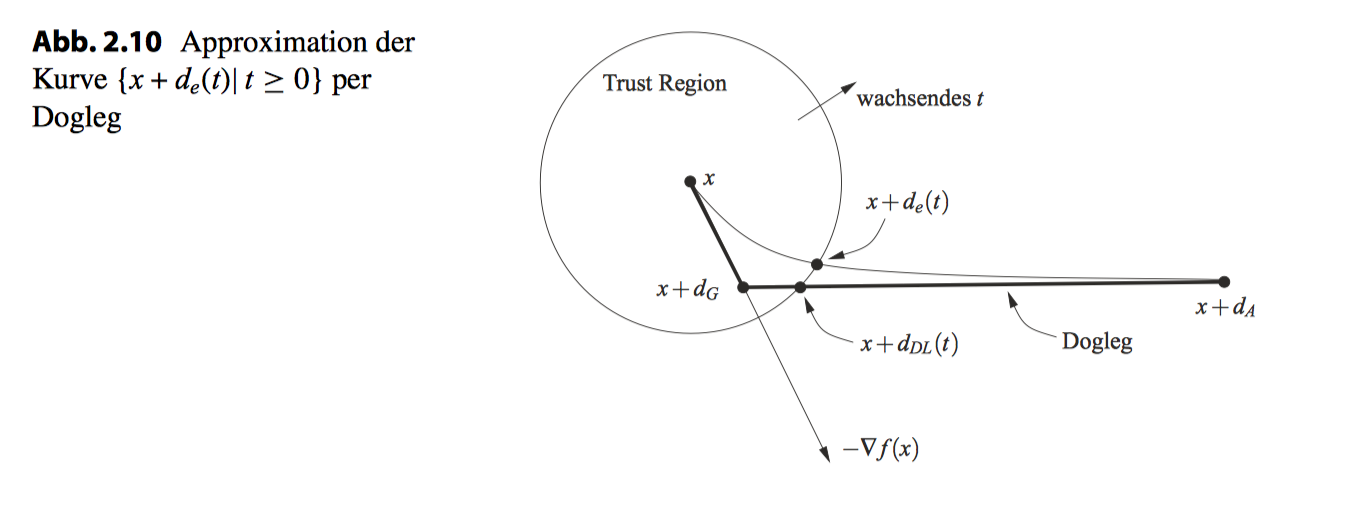
\includegraphics[scale=0.5]{ab210}
\end{center}

\begin{uebung}
	Es gilt für $A = A^T \succ 0$:
	\begin{enumerate}[label=\alph*\upshape)]
		\item $\|\hat{d}(s)\|_2$ ist monoton wachsend in $s$.
		\item $m(\hat{d}(s))$ ist monoton fallend in $s$.
	\end{enumerate}
\end{uebung}

Somit ergibt die Dogleg-Moethode die inexakte Lösung $x + d_{DL}(t)$ mit
$$ d_{DL} = \begin{cases}
 d_A, & \text{ falls } \| d_A \|_2 < t \\ \| s \cdot d_G \|_2 = t & \text{ falls } t < \| d_G \|_2 \\ \| d_G + (s - 1) (d_A - d_G) \|_2= t, & \text{ sonst}	
 \end{cases}
 $$
 
 \subsubsection*{Minimierung auf einem zweidimensionalen Teilraum}

Die inexakte Lösung von $TR$ durch die Dogleg-Methode kann verbessert werden, indem man $TR$ nicht auf den eindimensionalen Polygonzug einschränkt, sondern auf den zweidimensionalen Teilraum, der von d G und d A aufgespannt wird. In diesem Raum liegen insbesondere alle Punkte des Polygonzugs. Man erhält das Hilfsproblem

$$ \min_{d \in \mathbb{R}^n} m(d) \text{ s.t. } \| d \|_2 \leq t, ~ d \in \operatorname{bild}(\nabla f(x), A^{-1} \nabla f(x)) $$

Ein Hauptvorteil dieses Ansatzes besteht darin, dass er sich im Gegensatz zur DoglegMethode sinnvoll auf indefinite Matrizen A erweitern lässt. Für Details sei auf [25] verwiesen.

\chapter*{II. Restringierte Probleme}

\setcounter{chapter}{3}
\setcounter{section}{1}
\setcounter{thm}{0}

Wir betrachten im folgenden Problem
$$ P: \quad \min_{x \in \mathbb{R}^n} f(x) ~\text{ s.t. }~ g_i(x) \leq 0, i \in I, ~ h_j(x) = 0, j \in J $$
Mit von vektorwertigen Funktionen lässt sich die Menge $M$ der für $P$ zulässigen Punkte schreiben als
$$ M = \big\{ x \in \mathbb{R}^n ~|~ g(x) \leq 0, h(x) = 0 \big\} $$

\section*{Topologische Eigenschaften}

In Übung 1.2.11 haben wir bereits gesehen, dass $M$ unter der Stetigkeitsvoraussetzung an die Funktionen $g$ und $h$ eine abgeschlossene Menge ist.

\begin{definition}[Aktive-Index-Menge]
	Zu $\overline{x} \in M$ heißt
	$$ I_0(\overline{x}) = \big\{ i \in I ~|~ g_i(\overline{x}) = 0 \big\} $$
	Menge der aktiven Indizes oder auch \textbf{Aktive-Index-Menge}.
\end{definition}

\setcounter{thm}{2}

\begin{satz}
	Für jedes $\overline{x} \in M$ existiert eine Umgebung $U$ von $\overline{x}$ mit
	$$ U \cap M = U \cap \big\{ x \in \mathbb{R}^n ~|~ g_i(x) \leq 0, i \in I_0(\overline{x}), h_j(x) = 0, j \in J \big\} $$
\end{satz}

\begin{definition}[Zulässge Abstiegsrichtung]
	Gegeben sei das Problem
		$$ P: \quad \min f(x) \text{ s.t. } x \in M $$
	mit (nicht notwendigerweise in funktionaler Beschreibung vorliegender) zulässiger Menge $M \subseteq \mathbb{R}^n$. Dann heißt ein Vektor $d \in \mathbb{R}^n$ \textbf{zulässige Abstiegsrichtung} für $P$ in $\overline{x} \in M$, falls folgendes gilt
		$$ \exists \hat{t} > 0 ~\forall t \in (0, \hat{t}): \quad f(\overline{x} + td) < f(\overline{x}), ~\overline{x} + td \in M $$
\end{definition}

\begin{uebung}
	Für das Problem $P$ aus Definition 3.1.4 sei $\overline{x}$ ein lokaler Minimalpunkt. Dann existiert keine zulässige Abstiegsrichtung für $P$ in $\overline{x}$.
\end{uebung}

\begin{uebung}
	Gegeben sei das Problem
	$$ P: \quad \min f(x) \text{ s.t. } g_i(x) \leq 0, i \in I, h_j(x) = 0, j \in J $$
	Ein Vektor $d \in \mathbb{R}^n$ ist genau dann zulässige Abstiegsrichtung für $P$ in $\overline{x} \in M$, wenn folgendes gilt
	$$ \exists \hat{t} > 0 ~\forall t \in (0, \hat{t}: f(\overline{x} + td) < f(\overline{x}), \overline{x} + td \in M  $$
\end{uebung}

\begin{definition}[Äußerer Linearisierungskegel]
	Für $\overline{x} \in \mathbb{R}^n$ heißt 
		$$ L_{\leq}(\overline{x}, M) = \big\{ d \in \mathbb{R}^n ~|~\langle \nabla g_i(\overline{x}), d \rangle \leq 0, i \in I_0(\overline{x}) \big\} $$
	\textbf{äußerer Linearisierungksegel} an $M$ in $\overline{x}$.
\end{definition}

\begin{definition*}
	Eine Menge $A \subseteq \mathbb{R}^n$ wird als Kegel bezeichnet, wenn
	$$ \forall a \in A, \lambda > 0: \quad \forall \cdot a \in A $$
\end{definition*}

\begin{uebung}
	Am Punkt $\overline{x} \in M$ seien die Funktionen $g_i$, $i \in I_0(\overline{x})$, differenzierbar, dann ist $L_{\leq}(\overline{x}, M)$ ein konvexer Kegel.
\end{uebung}

Die funktionale Beschreibung einer zulässigen Menge kann so ungeschickt sein kann, dass ein äußerer Linearisierungskegel die lokale Struktur der Menge nicht notwendigerweise gut wiedergibt.

\setcounter{thm}{10}

\begin{definition}[Innerer Linearisierungskegel]
	Für $\overline{x} \in \mathbb{R}^n$ heißt
		$$ L_{<}(\overline{x}, M) = \big\{ d \in \mathbb{R}^n ~|~\langle \nabla g_i(\overline{x}), d \rangle < 0, i \in I_0(\overline{x}) \big\} $$
		\textbf{innerer Linearisierungskegel} an $M$ in $\overline{x}$.	
\end{definition}

\begin{definition}[Nichtdegenerierte funktionale Beschreibung einer Menge]
	Die funktionale Beschreibung von $M$ heißt an $\overline{x}$ \textbf{nichtdegeneriert}, wenn $\operatorname{cl} L_{<}(\overline{x}, M) = L_{\leq}(\overline{x}, M)$ gilt. Ansonsten heißt sie \textbf{degeneriert}. Diese Gleichheit ist auch als Cottle-Bedingung (Cottle constraint qualification) bekannt.
\end{definition}

\setcounter{thm}{14}

\begin{satz}
	Die funktionale Beschreibung von $M$ ist an $\overline{x}$ genau dann nichtdegeneriert, wenn $L_{<}(\overline{x}, M) \neq \emptyset$ gilt.	
\end{satz}

Es gibt zudem Fälle, in denen schon die Geometrie der zulässigen Menge so ungünstig ist, dass keine funktionale Beschreibung die gewünschte \enquote{gute} Approximation erster Ordnung liefert.

\begin{center}
	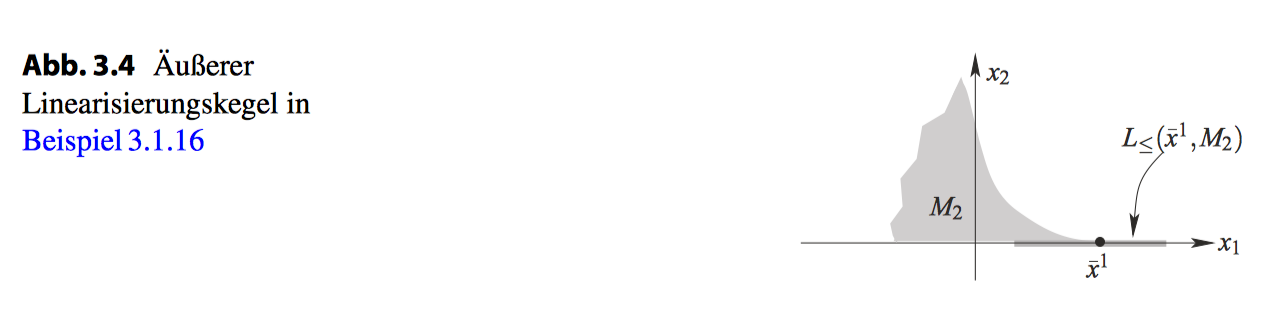
\includegraphics[scale=0.5]{ab34}
\end{center}

\setcounter{thm}{16}

\begin{definition}[Innerer und äußerer Tangentialkegel]
	Es seien $\overline{x} \in \mathbb{R}^n$ und $M \subseteq \mathbb{R}^n$. Eine Richtung $\overline{d} \in \mathbb{R}^n$ liegt im
	\begin{enumerate}[label=\alph*\upshape)]
		\item \textbf{inneren Tangentialkegel} $\Gamma(\overline{x}, M)$ an $M$ in $\overline{x}$, fall ein $\hat{t} > 0$ und eine Umgebung von $\overline{d}$ existieren mit 
			$$ \forall t \in (0, \hat{t}), d \in D: \quad \overline{x} +td \in M, $$
		\item \textbf{äußeren Tangentialkegel} $C(\overline{x}, M)$ an $M$ in $\overline{x}$, falls Folgen $(t^k)$ und $(d^k)$ existieren mit
			$$ t^k \searrow 0, d^k \rightarrow \overline{d}, ~\forall k \in \mathbb{N}: \quad \overline{x} + t^k d^k \in M $$
	\end{enumerate}	
\end{definition}

Der äußere Tangentialkegel ist im Gegensatz zum äußeren Linearisierungskegel nicht notwendigerweise konvex.

Abb. 3.5 zeigt Beispiele für innere und äußere Tangentialkegel sowie Vektoren $\overline{d}^1 \notin \Gamma(\overline{x}^1, M)$ und $\overline{d}^2 \in C(\overline{x}^2, M)$. Würde man in Definition 3.1.17 keine variablen Richtungen zulassen, so resultierte dies hingegen in $\overline{d}^1 \in \Gamma(\overline{x}^1, M)$ und $\overline{d}^2 \notin C(\overline{x}^2, M)$.

\begin{center}
	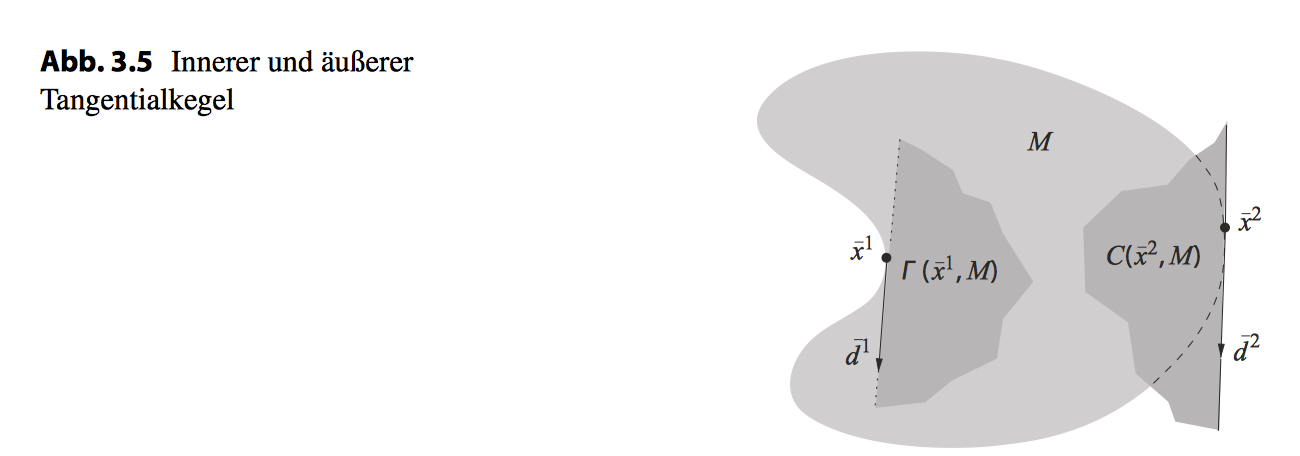
\includegraphics[scale=0.5]{ab35}
\end{center}

\begin{lemma}
	Es seien $\overline{x} \in \mathbb{R}^n$ und $M \subseteq \mathbb{R}^n$. Dann gilt:
	\begin{enumerate}[label=\alph*\upshape)]
		\item $\Gamma(\overline{x}, M) \subseteq C(\overline{x}, M)$.
		\item $\Gamma(\overline{x}, M)^C = C(\overline{x}, M^c)$.
		\item $\Gamma(\overline{x}, M)$ ist ein offener und $C(\overline{x}, M)$ ein abgeschlossener Kegel.
	\end{enumerate}
\end{lemma}

\begin{definition}[Nichtdegenerierte Geometrie einer Menge]
	Die Geometrie von $M$ heißt an $\overline{x}$ \textbf{nichtdegeneriert}, wenn $\operatorname{cl} \Gamma(\overline{x}, M) = C(\overline{x}, M)$ gilt. Ansonsten heißt sie \textbf{degeneriert}.
\end{definition}

\setcounter{thm}{23}

\begin{satz}
	Für alle $\overline{x} \in M$ gilt die Inklusions
	$$ L_{<}(\overline{x}, M) \subseteq \Gamma(\overline{x}, M) \subseteq C(\overline{x}, M) \subseteq L_{\leq}(\overline{x}, M). $$
\end{satz}

\setcounter{thm}{25}

\begin{korollar}
	Die funktionale Beschreibung der Menge $M$ sei an $\overline{x}$ nichtdegeneriert. Dann ist auch die Geometrie von $M$ an $\overline{x}$ nichtdegeneriert.
\end{korollar}

\section*{Optimalitätsbedingungen}

\subsection*{Stationarität}

\setcounter{section}{2}
\setcounter{thm}{0}

Da wir dabei nur die Geometrie von $M$ benutzen wollen, definieren wir Stationarität mit Hilfe einer geometrischen Approximation erster Ordnung, nämlich des äußeren Tangentialkegels.

\begin{definition}[Stationärer Punkt - restringierter Fall]
	Die Funktion $f \colon \mathbb{R}^n \rightarrow \mathbb{R}$ sei an $\overline{x} \in M$ differenzierbar. Dann heißt $\overline{x}$ stationärer Punkt von $P$, falls $\langle \nabla f(\overline{x}), d \rangle \geq 0$ für jede Richtung $d \in C(\overline{x}, M)$ gilt.
\end{definition}

\begin{satz}
	Die Funktion $f \colon \mathbb{R} \rightarrow \mathbb{R}$ sei an einem lokalen Minimalpunkt $\overline{x}$ von $P$ differenzierbar. Dann ist $\overline{x}$ stationärer Punkt im Sinne von Definition 3.2.1.	
\end{satz}

Hier nutzen wir aus, dass differenzierbare Funktionen auch einseitige richtungsdifferenzierbar im Sinne von Hadamard sind:
$$ \langle \nabla f(x), d) = \lim_k \frac{f(x + t^k d^k) - f(x)}{t^k} $$

\subsection*{Constraint Qualifications}

Diese Beobachtungen führen zur Definition von zwei Regularitätsbedingungen (constraint qualifications).

\begin{definition}[Abadie- und Mangasarian-Fromowitz-Bedingung für $J = \emptyset$]
	An $\overline{x} \in M$ gilt
	\begin{enumerate}[label=\alph*\upshape)]
		\item die \textbf{Abadie-Bedingung} (AB) für $J = \emptyset$, falls folgendes erfüllt ist
			$$ C(\overline{x}, M) = L_{\leq}(\overline{x}, M) $$
		\item die \textbf{Mangasarian-Fromowitz-Bedingung} (MFB) für $J = \emptyset$, falls folgendes gilt
			$$ L_{<}(\overline{x}, M) \neq \emptyset $$
	\end{enumerate}
\end{definition}

Nach Definition des inneren Linearisierungskegels ist die MFB an einem Punkt $\overline{x}$ genau dann erfüllt, wenn eine Richtung $d \in \mathbb{R}$ mit folgendem existiert
$$ \langle \nabla g_i(\overline{x}), d \rangle < 0, ~i \in I_0(\overline{x}) $$
Die MFB kann an einem Punkt bloß deshalb verletzt sein kann, weil die dort geometrisch nichtdegenerierte zulässige Menge degeneriert funktional beschrieben ist.

\begin{korollar}
	An einem lokalen Minimalpunkt $\overline{x}$ von $P$ seien $f$ und die Funktionen $g_i$, $i \in I_0(\overline{x})$ differenzierbar.
	\begin{enumerate}[label=\alph*\upshape)]
		\item Dann ist das folgende System mit keinem $d \in \mathbb{R}^n$ lösbar:
			\begin{equation}
				\langle \nabla f(\overline{x}), d \rangle < 0, ~\langle \nabla g_i(\overline{x}), d \rangle < 0 \quad i \in I_0(\overline{x}) \tag*{(3.1)}
			\end{equation} 
		\item Falls an $\overline{x}$ die AB gilt, dann ist sogar das folgende System mit keinem $d \in \mathbb{R}^n$ lösbar:
			\begin{equation}
				\langle \nabla f(\overline{x}), d \rangle < 0, ~ \langle \nabla g_i(\overline{x}), d \rangle \leq 0 \quad i \in I_0(\overline{x}) \tag*{(3.2)}
			\end{equation} 
	\end{enumerate}
\end{korollar}

\begin{uebung}
	Zu $\overline{x} \in M$ jede Richtung $d$ mit (3.1) ist eine zulässige Abstiegsrichtung in $\overline{x}$ im Sinne von Definition 3.1.4, und zwar sowohl für $P$ als auch für das linearisierte Problem $P_{lin}(\overline{x})$.
\end{uebung}

\begin{uebung}
	Zu $\overline{x} \in M$ ist jede Richtung $d$ mit (3.2) eine zulässige Abstiegsrichtung für $P_{lin}(\overline{x})$ in $\overline{x}$ im Sinne von Definition 3.1.4 ist.
\end{uebung}
 
 Stationarität schließt sogar die Existenz gewisser unzulässiger Abstiegsrichtungen aus. Da die notwendige Bedingung aus Korollar 3.2.4a bei verletzter $MFB$ trivialerweise erfüllt sein kann, werden wir im Folgenden versuchen, die Bedingung aus Korollar 3.2.4b algorithmisch zu verwerten. Dazu ist es zunächst erforderlich, an einem Punkt $\overline{x} \in M$ algorithmisch nachprüfbare hinreichende Bedingungen für die Gültigkeit der abstrakt formulierten $AB$ zu kennen.
 
\setcounter{thm}{7}

\begin{satz}
	An jedem $\overline{x} \in M$ impliziert die MFB die AB.	
\end{satz}

\begin{uebung}
	Die Funktion $f \colon \mathbb{R}^n \rightarrow \mathbb{R}$ sei an $\overline{x}$ differenzierbar mit $\nabla f(\overline{x}) \neq 0$, dann
	$$ C \left( \overline{x}, f_{\leq}^{f(\overline{x})} \right) = \big\{ d \in \mathbb{R}^n ~|~ \langle \nabla f(\overline{x}), d \rangle \leq 0 \big\} $$
\end{uebung} 
 Neben Satz 3.2.8 motiviert sich eine andere wichtige hinreichende Bedingung für die Gültigkeit der AB aus der Tatsache, dass die AB eine Linearisierungseigenschaft der zulässigen Menge fordert, die dann erfüllt sein sollte, wenn die Menge ohnehin schon durch endlich viele lineare Ungleichungen beschrieben ist. In diesem Fall nennt man $M$ polyedrisch.
 
\begin{beispiel}
	Für alle $1 \leq i \leq p$ sei
$$g_i(x) =a_i^T x + b_i $$
	mit $a_i \in \mathbb{R}^n$, $b_i \in \mathbb{R}$. In Matrix-Vektor-Schreibweise ist $g(x) \leq 0$ dann gleichbedeutend mit der aus der linearen Optimierung bekannten Restriktion $Ax + b \leq 0$. Hier ist $AB$ automatisch erfüllt.	
\end{beispiel}

Falls also $\overline{x} \in M$ ein lokaler Minimalpunkt einer dort differenzierbaren Funktion $f$ über einer so definierten Menge $M$ ist, dann lässt sich laut Korollar 3.2.4b das System

	$$	\langle \nabla f(\overline{x}), d \rangle < 0, ~\langle a_i, d \rangle \leq 0, ~ i \in I_0(\overline{x})	$$

mit keinem $d \in \mathbb{R}^n$ lösen.
 
\setcounter{thm}{11}
 
\begin{uebung}
	In der Beschreibung der Menge $M = \{ x \in \mathbb{R}^n ~|~ g_i(x) \leq 0, i \in I\}$ seien alle Funktionen $g_i$, $i \in I$, konkav auf $\mathbb{R}^n$. Zeigen Sie, dass dann die $AB$ an jedem Punkt von $M$ gilt.
\end{uebung}

\subsection*{Alternativsätze}
 
Geometrisch bedeutet die Bedingung in Korollar 3.2.4a
$$ \langle a^k, d \rangle < 0 \quad 1 \leq k \leq r,$$  dass es keinen Vektor $d$ gibt, der gleichzeitig mit allen Vektoren $a_1, \dotsc , a_r$ einen stumpfen Winkel bildet.
 
\begin{center}
	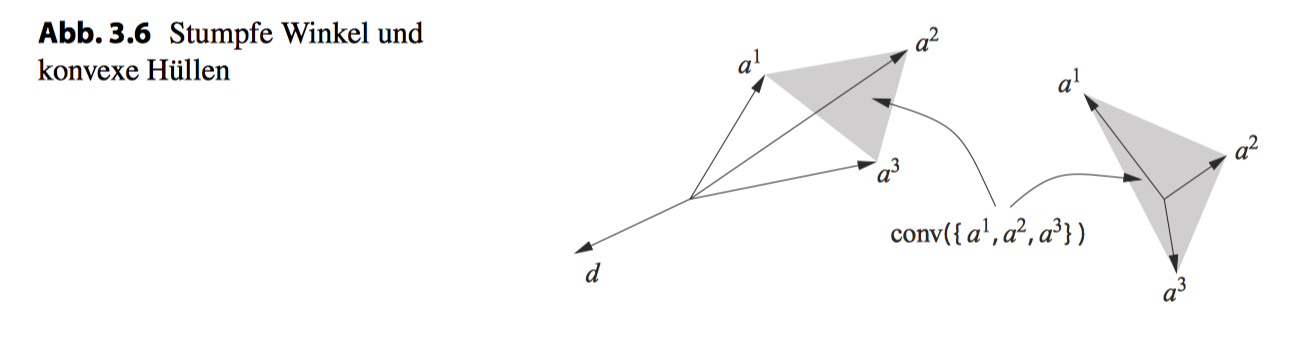
\includegraphics[scale=0.5]{ab36}
\end{center} 
 
In Abb. 3.6 sind rechts drei Vektoren eingezeichnet, für die dies der Fall ist, während links ein Vektor $d$ existiert, der mit allen drei Vektoren gleichzeitig einen stumpfen Winkel bildet. Ebenfalls eingezeichnet ist die konvexe Hülle dieser drei Vektoren. Allgemein besteht die konvexe Hülle conv(A) einer Menge $A \subseteq \mathbb{R}^n$ aus der Menge aller Konvexkombinationen von Elementen in $A$. In Abb. 3.6 beobachtet man, dass die Unlösbarkeit des Ungleichungssystems (rechts) damit einhergeht, dass der Nullpunkt in der konvexen Hülle der drei Vektoren enthalten ist, während dies bei Lösbarkeit des Ungleichungssystems (links) nicht der Fall ist. Dass dies tatsächlich immer so ist, führt letztlich auf algorithmisch verwertbare Optimalitätsbedingungen und ist der Inhalt des folgenden zentralen Resultats, dessen vollständiger Beweis einiger Vorbereitung bedarf.
 
\begin{lemma}
	Für Vektoren $a^k \in \mathbb{R}^n$, $1 \leq k \leq r$, mit $r \in \mathbb{N}$ gilt genau eine der beiden folgenden Alternativen.
	\begin{enumerate}[label=\alph*\upshape)]
		\item Das System $\langle a^k, d \rangle < 0$, $1 \leq k \leq r$, hat eine Lösung $d \in \mathbb{R}^n$.
		\item Es gilt $0 \in \operatorname{conv}(\{ a^1, \dotsc, a^r \})$.
	\end{enumerate}
\end{lemma} 

\begin{satz}[Trennungssatz] Es seien $X \subseteq \mathbb{R}^n$ eine nichtleere, abgeschlossene und konvexe Menge sowie $z \in X^c$. Dann existieren ein $a \in \mathbb{R}^n \setminus \{ 0 \}$ und ein $b \in \mathbb{R}$, so dass für alle $x \in X$ die folgende Ungleichungen erfüllt sind:
	$$ \langle a, x \rangle \leq b < \langle a, z \rangle $$
\end{satz}
 
\begin{definition*}
	\begin{enumerate}[label=\alph*\upshape)]
		\item Konvexe Hülle $\operatorname{conv}(A) = \big\{ \sum_{i=1}^s \lambda_i a^i ~|~ a^i \in A, \lambda_i \geq 0, \sum \lambda_i = 1, 1 \leq i \leq s, s \in \mathbb{N} \big\}$
		\item Konvexe Kegelhülle $\operatorname{cone}(A) = \big\{ \sum_{i=1}^s \lambda_i a^i ~|~ a^i \in A, \lambda_i \geq 0, 1 \leq i \leq s, s \in \mathbb{N} \big\}$
	\end{enumerate}	
\end{definition*}
 
\begin{satz}[Lemma von Farkas] 
	Für Vektoren $a^k \in \mathbb{R}^n$, $0 \leq k \leq r$, mit $r \in \mathbb{R}$ gilt genau eine der beiden folgenden Alternativen.
	\begin{enumerate}[label=\alph*\upshape)]
		\item Das System $\langle a^0, d \rangle < 0, \langle a^k, d \rangle \leq 0$, $1 \leq k \leq r$ hat eine Lösung $d \in \mathbb{R}^n$.
		\item Es gilt $-a^0 \in \operatorname{cone}(\{a^1, \dotsc, a^r \})$
	\end{enumerate}
\end{satz}

\begin{center}
	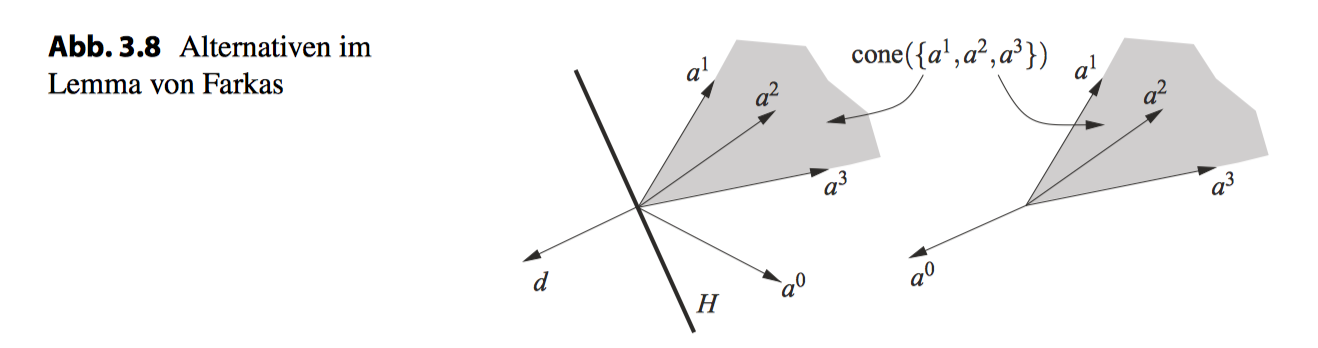
\includegraphics[scale=0.5]{ab38}
\end{center}
 
\begin{satz}[Satz von Carathéodory]
	Für jede Menge $A \subseteq \mathbb{R}^n$ gelten die folgenden Aussagen:
	\begin{enumerate}[label=\alph*\upshape)]
		\item Zu jedem $\overline{x} \in \operatorname{cone}(A) \setminus \{ 0 \}$ existieren ein $r \leq n$ und linear unabhängige $x^k \in A$ sowie $\lambda_k > 0$, $1 \leq k \leq r$ mit $\overline{x} = \sum_{k=1}^r \lambda_k x^k$.
		\item Zu jedem $\overline{x} \in \operatorname{conv}(A)$ existieren ein $r \leq n + 1$ und $x^1, \dotsc, x^r \in A$, so dass die Vektoren $x^2 - x^1, \dotsc, x^r - x^1$ linear unabhängig sind und dass $\overline{x} \in \operatorname{conv}(\{ x^1, \dotsc, x^r \})$ gilt.
	\end{enumerate}
\end{satz} 
 
Die in Satz 3.2.16b auftretende konvexe Hülle $\operatorname{conv}(\{x_1 , \dotsc , x_r \})$ von $r$ Punkten mit linear unabhängigen Vektoren $x^2 - x^1 , \dotsc, x^r - x^1$ wird auch $(r - 1)$-Simplex genannt, und die Vektoren $x^1, \dotsc, x^r$ heißen dann affin unabhängig. ~\bigskip

Der Satz von Carathéodory liefert sofort die folgenden Verbesserungen der Aussagen im Lemma von Gordan und im Lemma von Farkas, wobei $|A|$ die Anzahl der Elemente einer Menge $A$ bezeichne. 

\begin{korollar} ~\
	\begin{enumerate}[label=\alph*\upshape)]
		\item In Satz 3.2.13b lassen sich Gewichte $\lambda_k$ mit $|\{ 1 \leq k \leq r ~|~\lambda_k > 0\}| \leq n+1$ wählen.
		\item In Satz 3.2.15b lassen sich Gewichte $\lambda_k$ mit $|\{ 1 \leq k \leq r ~|~\lambda_k > 0\}| \leq n$ wählen.
	\end{enumerate}
\end{korollar}

\subsection*{Optimalitätsbedingungen erster Ordnung ohne Gleichungsrestriktionen}

\begin{satz}[Satz von Fritz John für $J = \emptyset$]
	Es sei $\overline{x}$ ein lokaler Minimalpunkt von $P$, an dem die Funktionen $f$ und $g_i$, $i \in I_0(\overline{x})$, differenzierbar sind. Dann existieren Multiplikatoren $\kappa \geq 0$, $\lambda_i \geq 0$, $i \in I_0(\overline{x})$, nicht alle null, mit
	\begin{equation}
		\kappa \nabla f(\overline{x}) + \sum_{i \in I_0(\overline{x})} \lambda_i \nabla g_i(\overline{x}) = 0 \tag*{(3.3)}
	\end{equation} 
	Dabei kann man $\kappa$ und die $\lambda_i$ so wählen, dass entweder $\kappa > 0$ und $|\{ i \in I_0(\overline{x}) ~|~\lambda_I > 0 \} | \leq n$ gilt oder $\kappa = 0$ und $|\{ i \in I_0(\overline{x}) ~|~\lambda_i > 0 \} | \leq n + 1$.
\end{satz}
 
Die Beschränkung der Anzahl positiver Multiplikatoren in der zweiten Behauptung aus Satz 3.2.18 zieht nach sich, dass die $|I_0(x)| \leq n + 1$. ~\bigskip
 
Zur Motivation der MFB in Definition 3.2.3 haben wir angeführt, dass die im Beweis zu Satz 3.2.18 benutzte Unlösbarkeit des Systems trivialerweise erfüllt sein kann, wenn nämlich $L_< (x, M) = \emptyset$ gilt. 
 
\setcounter{thm}{20}

\begin{lemma}
	Es sei $\overline{x}$ ein lokaler Minimalpunkt von $P$, an dem die Funktionen $f$ und $g_i$ , $i \in I_0(\overline{x})$, differenzierbar sind. Dann ist (3.3), also
	$$ \kappa \nabla f(\overline{x}) + \sum_{i \in I_0(\overline{x})} \lambda_i \nabla g_i(\overline{x}) = 0, $$
	 genau dann mit $\kappa = 0$ erfüllbar, wenn die $MFB$ an $\overline{x}$ verletzt ist.
\end{lemma}

\begin{satz}[Satz von Karush-Kuhn-Tucker für $J = \emptyset$ unter $MFB$] 
	Es sei $\overline{x}$ ein lokaler Minimalpunkt von $P$, an dem die Funktionen $f$ und $g_i$, $i \in I_0(\overline{x})$, differenzierbar sind, und an $\overline{x}$ gelte die $MFB$. Dann existieren Multiplikatoren $\lambda_i \geq 0$, $i \in I_0(\overline{x})$ mit
	  $$ \nabla f(\overline{x}) + \sum_{i \in I_0(\overline{x})} \lambda_i \nabla g_i(\overline{x}) = 0 $$
	Dabei kann man die $\lambda_i$ so wählen, dass $|\{ i \in I_0 (\overline{x}) ~|~\lambda_i > 0 \}| \leq n$ gilt.
\end{satz}

\begin{satz}[Satz von Karush-Kuhn-Tucker für $J = \emptyset$ unter $AB$]
	Die Aussage von Satz 3.2.22 bleibt richtig, wenn man dort \enquote{$MFB$} durch \enquote{$AB$} ersetzt.
\end{satz}

\begin{korollar}
	Es seien $g_i(x) = a_i^T x + b_i$, $1 \leq i \leq p$, und $\overline{x}$ sei ein lokaler Minimalpunkt von $P$, an dem $f$ differenzierbar ist. Dann existieren Multiplikatoren $\lambda_i \geq 0$, $i \in I_0(\overline{x})$ mit
	$$  $$
	Dabei kann man die $\lambda_i$ so wählen, dass $|\{ i \in I_0(\overline{x})| \lambda_i > 0 \}| \leq n$ gilt.
\end{korollar}
 
\subsection*{Trennungssatz}

\begin{lemma}
	Es seien $X \subseteq \mathbb{R}^n$ eine nichtleere abgeschlossene Menge und $z \in \mathbb{R}^n$. Dann ist das Projektionsproblem 
	$$ Pr(z, X): \quad \min \| x - z \|_2 \text{ s.t. } x \in X $$
	lösbar.
\end{lemma}

\begin{satz}
	Es seien $X \subseteq \mathbb{R}^n$ eine nichtleere, abgeschlossene und konvexe Menge sowie $z \in \mathbb{R}^n$. Dann besitzt das Problem $Pr(z, X)$ einen eindeutigen globalen Minimalpunkt.	
\end{satz}

\begin{satz}[Variationsformulierung konvexer Probleme]
	Die Menge $M \subseteq \mathbb{R}^n$ und die Funktion $f \in C^1(M, \mathbb{R})$ seien konvex. Dann gelten die folgenden Aussagen:
	\begin{enumerate}[label=\alph*\upshape)]
		\item Der Punkt $\overline{x} \in \mathbb{R}^n$ ist genau dann globaler Minimalpunkt von
				$$ P: \quad \min f(x) \text{ s.t. } x \in M, $$
			wenn $\overline{x}$ globaler Minimalpunkt von folgendem ist
			 $$ \tilde{P}_{lin}(\overline{x}): \quad \min_x \langle \nabla f(\overline{x}), x - \overline{x} \rangle \text{ s.t. } x \in M $$
		\item Die Menge der globalen Minimalpunkte von $P$ stimmt mit der folgenden Menge überein
			$$ \big\{ \overline{x} \in M ~|~  \langle \nabla f(\overline{x}), x - \overline{x} \rangle \geq 0 \text{ für alle } x \in M \big\} $$
	\end{enumerate}	
\end{satz}

\begin{definition}[Normalenkegel an konvexe Mengen]
	Für eine konvexe Menge $X \subseteq \mathbb{R}^n$ und $\overline{x} \in X$ heißt
		$$ N(\overline{x}, X) \coloneqq \big\{ s \in \mathbb{R}^n ~|~\langle s, x - \overline{x} \rangle \leq 0 \text{ für alle } x \in X \big\} $$ \textbf{Normalenkegel} an $X$ in $\overline{x}$. Die Elemente $s$ des \textbf{Normalenkegels} $N(\overline{x}, X)$ nennt man auch (äußere) Normalenrichtungen an $X$ in $\overline{x}$.
\end{definition}
 
\begin{uebung}
	für jede (nicht notwendigerweise konvexe) Menge $X \subseteq \mathbb{R}^n$ und jedes $\overline{x} \in X$, dass die Menge $N(\overline{x}, X)$ ein konvexer und abgeschlossener Kegel mit $0 \in N(\overline{x}, X)$ ist.
\end{uebung} 

Geometrisch interpretiert liegen im Normalenkegel an $X$ in $x$ genau diejenigen Richtungen $s \in \mathbb{R}^n$, mit denen kein Vektor $d$ einen spitzen Winkel bindet, für den $x+d$ in $X$ liegt (was man mittels des Zusammenhangs $x = x + d$ sieht).
 
\begin{korollar}
	Die Menge $M \subseteq \mathbb{R}^n$ und die Funktion $f \in C^1(M, \mathbb{R})$ seien konvex. Dann ist $\overline{x} \in \mathbb{R}^n$ genau dann globaler Minimalpunkt von
		$$ P: \quad \min f(x) \text{ s.t. } x \in M $$
	wenn die Bedingungen $\overline{x} \in X$ und $- \nabla f(\overline{x}) \in N(\overline{x}, X)$ erfüllt sind.
\end{korollar} 
 
\begin{satz}[Projektionslemma]
	Es seien $X \subseteq \mathbb{R}^n$ eine nichtleere, abgeschlossene und konvexe Menge sowie $z \in \mathbb{R}^n$. Dann ist der eindeutige Minimalpunkt $pr(z, X)$ des Projektionsproblems
		$$ Pr(z, X): \quad \min \| x - z \|_2 \text{ s.t. } x \in X $$
	gleichzeitig die eindeutige Lösung der Bedingungen
		$$ x \in X \text{ und } z \in x + N(x, X) $$
\end{satz}

\subsection*{Normalenkegel}

\setcounter{thm}{32}

\begin{definition}[Polarkegel]
	 Für eine Menge $A \subseteq \mathbb{R}^n$ heißt
		$$ A^\circ = \big\{ s \in \mathbb{R}^n ~|~\langle s, d \rangle \leq 0 \text{ für alle } d \in A \big\} $$
	\textbf{Polarkegel} von $A$.
\end{definition}

Dabei gilt für eine konvexe Menge $X$, dass der Normalenkegel wie folgt lautet: 
	$$ N(\overline{x}, X) = (X - \overline{x})^\circ. $$
Für eine beliebige Menge $X$ benutzen wir stattdessen den Polarkegel des äußeren Tangentialkegels als Normalenkegel.

\begin{definition}[Normalenkegel an beliebige Mengen]
	Für eine Menge $X \subseteq \mathbb{R}^n$ und $\overline{x} \in X$ heißt
		$$ N(\overline{x}, X) = C^{\circ}(\overline{x}, X) $$
	\textbf{Normalenkegel} an $X$ in $\overline{x}$. Die Elemente $s$ des Normalenkegels $N(\overline{x}, X)$ heißen wieder (äußere) Normalenrichtungen an $X$ in $\overline{x}$. 
\end{definition}
 
\begin{satz}
	Für jede konvexe Menge $X \subseteq \mathbb{R}^n$ und $\overline{x} \in X$ gilt
	$$ (X - \overline{x})^\circ = C^\circ(\overline{x}, X) $$
\end{satz}

Satz 3.2.2 besagt in dieser Terminologie tatsächlich, dass an einem lokalen Minimalpunkt $\overline{x}$ von $f$ auf $M$ notwendigerweise die Beziehung

 $$ - \nabla f(\overline{x}) \in N(\overline{x}, M) $$

gilt. Die Stationaritätsbedingung kann man geometrisch also auch so interpretieren, dass an jedem lokalen Minimalpunkt $\overline{x}$ von $P$ der Vektor $-\nabla f(\overline{x})$ (also die steilste Abstiegsrichtung für $f$ in $\overline{x}$) eine äußere Normalenrichtung an $M$ in $\overline{x}$ ist. ~\bigskip

Da die funktionale Beschreibung der Menge $M$ für dieses Ergebnis keine Rolle spielt (sondern nur ihre Geometrie), waren für seine Herleitung keine Constraint Qualifications erforderlich. Im Folgenden werden wir aber sehen, wie sie bei der Herleitung einer expliziten Darstellung der Elemente des Normalenkegels helfen.

\begin{uebung}
	Für alle $\overline{x} \in M$ gilt die Inklusion $L_{\leq}^\circ(\overline{x}, M) \subseteq N(\overline{x}, M)$.
\end{uebung}

\begin{uebung}
	Mit Hilfe des Lemmas von Farkas gilt die folgende Identität für alle $\overline{x} \in M$
	$$ L_{\leq}^\circ(\overline{x}, M) = \operatorname{cone}(\{ \nabla g_i(\overline{x}), i \in I_0(\overline{x}) \}) $$
\end{uebung}

\begin{uebung}
	An $\overline{x} \in M$ gelte die AB. Wegen Übung 3.2.36 und Übung 3.2.37 gilt die Identität
	$$ N(\overline{x}, M) = \operatorname{cone}(\{ \nabla g_i(\overline{x}), i \in I_0(\overline{x}) \}) $$
\end{uebung}

Somit gilt für jeden lokalen Minimalpunkt $x$ von $P$, an dem die AB erfüllt ist, d.h.
$$ -\nabla f(x) \in \operatorname{cone}(\{ \nabla g_i(x), i \in I_0(x) \}), $$
also gerade die Behauptung des Satzes von Karush-Kuhn-Tucker.

\subsection*{Optimalitätsbedingungen erster Ordnung mit Gleichungsrestriktionen}
 
Von jetzt an sei die zulässige Menge von $P$ wieder durch  Ungleichungen und Gleichungen beschrieben, d. h., es gelte

$$ M = \big\{ x \in \mathbb{R}^n ~|~ g_i(x) \leq 0, i \in I, h_j(x) = 0, j \in J \big\}. $$
 
\begin{satz}
	Es sei $\overline{x}$ ein lokaler Minimalpunkt von $P$, an dem die Funktionen $f, g_i$, $i \in I_0(\overline{x})$, und $h_j$, $j \in J$, stetig differenzierbar sind. Dann existieren Multiplikatoren $\kappa \geq 0, \lambda_i \geq 0, i \in I_0(\overline{x}), \mu_j \in \mathbb{R}, j \in J$, nicht alle null, mit

		$$ \kappa \nabla f(\overline{x}) + \sum_{i \in I_0(\overline{x})} \lambda_i \nabla g_i(\overline{x}) + \sum_{j \in J} \mu_j \nabla h_j(\overline{x}) = 0 $$

	Dabei kann man $\kappa$ und die $\lambda_i$ so wählen, dass entweder $\kappa > 0$ und $|\{ i \in I_0(\overline{x}) ~|~ \lambda_i > 0 \}| \leq n - q$ gilt oder $\kappa = 0$ und $|\{ i \in I_0(\overline{x}) ~|~ \lambda_i > 0 \}| \leq n - q + 1$.
\end{satz} 

\begin{definition}[Mangasarian-Fromowitz-Bedingung]
	Der Punkt $\overline{} \in M$ erfüllt die Mangasarian-Fromowitz-Bedingung (MFB), falls folgende Bedingungen gelten:
	\begin{enumerate}[label=\alph*\upshape)]
		\item Die Vektoren $\nabla h_j(\overline{x}), j \in J$, sind linear unabhängig,
		\item Es existiert ein $d \in \mathbb{R}^n$ mit $\langle \nabla g_i(\overline{x}), d \rangle < 0, i \in I_0(\overline{x}), ~\langle \nabla h_j(\overline{x}), d \rangle = 0, j \in J$
	\end{enumerate}
\end{definition}
 
\begin{satz}[Satz von Karush-Kuhn-Tucker]
	Es sei $\overline{x}$ ein lokaler Minimalpunkt von $P$, an dem die Funktionen $f, g_i$, $i \in I_0(\overline{x})$, und $h_j$, $j \in J$, stetig differenzierbar sind, und an $\overline{x}$ gelte die $MFB$. Dann existieren Multiplikatoren $\lambda_i \geq 0$, $i \in I_0(\overline{x})$, $\mu_j \in \mathbb{R}$, $j \in J$, mit
	
		$$ \nabla f(\overline{x}) + \sum_{i \in I_0(\overline{x})} \lambda_i \nabla g_i(\overline{x}) + \sum_{j \in J} \mu_j \nabla h_j(\overline{x}) = 0 $$

	Dabei kann man die $\lambda_i$ so wählen, dass $|\{ i \in I_0(\overline{x}) ~|~ \lambda_i > 0 \}| \leq n - q$ gilt.	
\end{satz}

\begin{definition}[Lineare-Unabhängigkeits-Bedingung]
	An $\overline{x} \in M$ gilt die Lineare-Unabhängigkeits-Bedingung (LUB), falls die Vektoren $\nabla g_i(\overline{x})$, $i \in I_0(\overline{x})$, $\nabla h_j(\overline{x})$, $j \in J$, also die Gradienten aller in $\overline{x}$ aktiven Restriktionen, linear unabhängig sind.
\end{definition}
 
Das heißt insbesondere, dass falls nur eine Restriktion herrscht, diese im Punkt nicht identisch $0$ ist. 
 
\begin{satz}
	Die LUB an $\overline{x}$ impliziert die MFB an $\overline{x}$.	
\end{satz}

\setcounter{thm}{44}

\begin{beispiel}
	Die Spektralnorm einer Matrix entspricht dem KKT-Multiplikator $\mu$.
\end{beispiel}


\begin{bemerkung}
	Jede Zahl zu $\lambda$ einem positiven Eigenwert $\lambda$ der Matrix $A^TA$ heißt Singulärwert der $(m, n)$-Matrix $A$.	
\end{bemerkung}

\subsection*{Karush-Kuhn-Tucker-Punkte}
 
Der grundlegende Satz 3.2.41 erlaubt es, das aus dem unrestringierten Fall bekannte Konzept eines kritischen Punkts von $P$ auf den restringierten Fall zu übertragen.

\begin{definition}[Karush-Kuhn-Tucker-Punkt]
	Zu $\overline{x} \in M$ gebe es $\lambda_i \geq 0$, $i \in I_0(\overline{x})$, $\mu_j \in \mathbb{R}$, $j \in J$ mit
		$$ \nabla f(\overline{x}) + \sum_{i \in I_0(\overline{x})} \lambda_i \nabla g_i(\overline{x}) + \sum_{j \in J} \mu_j \nabla h_j(\overline{x}) = 0 $$
	Dann heißt $\overline{x}$ Karush-Kuhn-Tucker-Punkt (KKT-Punkt) von $P$. Die Koeffizienten $\lambda_i$, $i \in I_0(\overline{x})$, und $\mu_j$ j $\in J$ heißen KKT-Multiplikatoren. 
\end{definition}

Aus Ergebnissen der linearen Algebra folgt, dass die Multiplikatoren eines KKT-Punkts $\overline{x}$ eindeutig bestimmt sind, wenn an $\overline{x}$ die LUB gilt. Satz 3.2.41 und Satz 3.2.43 liefern daher folgendes Ergebnis.

\begin{korollar}
	Es sei $\overline{x}$ ein lokaler Minimalpunk von $P$, an dem die Funktionen $f$, $g_i$, $i \in I_0(\overline{x})$ und $h_j$, $j \in J$, stetig differenzierbar sind, und an $\overline{x}$ gelte die LUB. Dann ist $\overline{x}$ ein KKT-Punkt von $P$ mit eindeutigen KKT-Multiplikatoren.
\end{korollar}

\begin{center}
	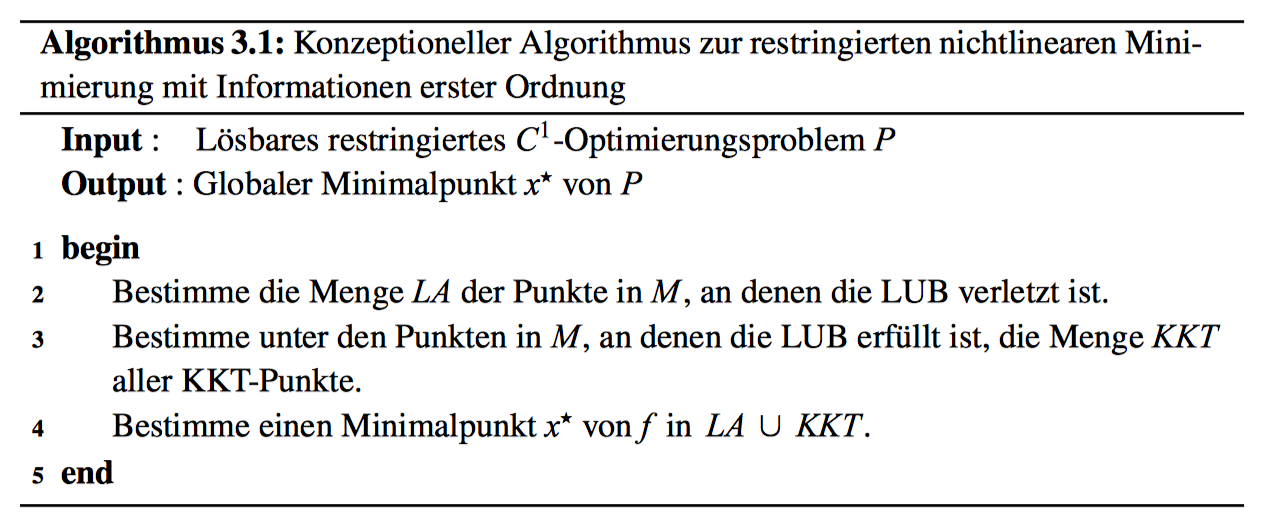
\includegraphics[scale=0.5]{a31}
\end{center}
 
Für kleine Werte von $p$ löst man durch Fallunterscheidung der aktiven Indexmenge das System

\begin{equation}
	\begin{rcases}
	\nabla f(x) + \sum_{i \in I_0(x)} \lambda_i \nabla g_i(x) + \sum_{j \in J} \mu_j \nabla h_j(x) & = 0, \\
	g_i(x) & \leq 0, i \in I, \\
	h_j(x) & = 0, j \in J, \\
	\lambda_i & \geq 0, i \in I_0(x).
\end{rcases} \tag*{(3.8)}
\end{equation}

Ist $p$ allerdings groß, schlägt man einen anderen Weg ein und löst das folgende System mit einer Komplementaritätsbedingung:

\begin{equation}
	\begin{rcases}
	\nabla f(x) + \sum_{i \in I} \lambda_i \nabla g_i(x) + \sum_{j \in J} \mu_j \nabla h_j(x) & = 0, \\
	g_i(x) & \leq 0, i \in I, \\
	h_j(x) & = 0, j \in J, \\
	\lambda_i & \geq 0, i \in I. \\
	\lambda_i \cdot g_i(x) & = 0, i \in I
\end{rcases} \tag*{(3.9)}
\end{equation}

Man fasst die letzte Zeile nicht zu $\sum_{i \in I} \lambda_i g_i(x) = 0$ zusammen, da dies später zu Problemen führt.

\begin{definition}[Strikte Komplementaritätsbedingung]
	Am KKT-Punkt $\overline{x}$ gelte die LUB, und zu $\overline{x}$ sei ($\overline{\lambda}_{I_0}, \overline{\mu})$ die eindeutige Lösung von (3.8). Dann gilt an $\overline{x}$ die strikte Komplementaritätsbedingung (SKB), falls $\overline{\lambda}_i > 0$ für alle $i \in I_0(\overline{x})$ erfüllt ist.
\end{definition}
 
Strikte Komplementarität bedeutet hier gerade, dass die Knickstelle dieser Menge, nämlich der Nullpunkt, aus der Menge entfernt wird.

\begin{center}
	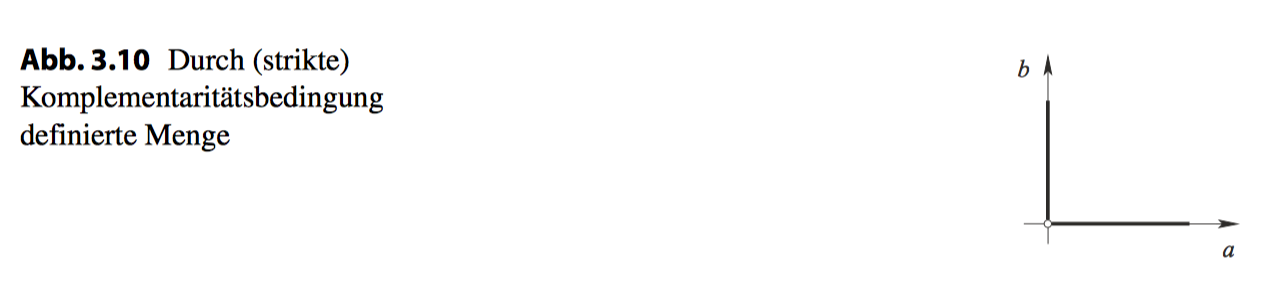
\includegraphics[scale=0.5]{ab310}
\end{center}

\setcounter{thm}{51}
 
\begin{definition}[Lagrange-Funktion]
	Die Funktion
	$$ L \colon \mathbb{R}^n \times \mathbb{R}^p \times \mathbb{R}^q \rightarrow \mathbb{R}, ~ (x, \lambda, \mu) \mapsto f(x) + \sum_{i \in I} \lambda_i g_i(x) + \sum_{j \in J} \mu_j h_j(x) $$
	heißt \textbf{Lagrange-Funktion} von $P$.
\end{definition} 

\subsection*{Optimalitätsbedingung zweiter Ordnung}

Um die Form der Optimalitätsbedingungen zweiter Ordnung in der restringierten Optimierung zu motivieren, betrachten wir die Gleichung, die aus $(3.11)$ durch Unterschlagen der Ungleichung entsteht:
$$ 0 = \mathfrak{T}(x, \lambda, \mu) \coloneqq \begin{pmatrix}
	\nabla_x L(x, \lambda, \mu) \\ \operatorname{diag}(\lambda) \cdot \nabla_\lambda L(x, \lambda, \mu) \\\
	\nabla_\mu L(x, \lambda, \mu)
\end{pmatrix} $$

\setcounter{thm}{54}

\begin{definition}[Kritischer Punkt eines restringierten Problems]
	Ein Punkt $\overline{x} \in M$, der mit Multiplikatorem $\overline{\lambda}$ und $\overline{\mu}$ die Gleichung $\mathfrak{T}(\overline{x}, \overline{\lambda}, \overline{\mu}) = 0$ erfüllt, heißt\textbf{kritischer Punkt} von $P$.
\end{definition}


Kritische Punkte unterscheiden sich von KKT-Punkten nur dadurch, dass keine Nichtnegativitätsbedingung an $\overline{x}$ gefordert wird.

\setcounter{thm}{56}

\begin{lemma}
	Es sei $\mathfrak{T}(\overline{x}, \overline{\lambda}, \overline{\mu}) = 0$. Dann ist $D \mathfrak{T}(\overline{x}, \overline{\lambda}, \overline{\mu})$ genau dann nichtsingulär, wenn $\overline{\lambda}_i \neq 0$ für alle $i \in I_0(\overline{x})$ gilt und wenn die folgende Matrix nichtsingulär ist
	$$ \begin{pmatrix}
		D^2_x L(\overline{x}, \overline{\lambda}, \overline{\mu}) & \nabla g_{I_0}(\overline{x}) & \nabla h(\overline{x}) \\ D g_{I_0}(\overline{x}) & 0 & 0 \\
		D h(\overline{x}) & 0 & 0
	\end{pmatrix} $$
\end{lemma}

\begin{definition}[Einschränkung einer Matrix]
	Die $(n-m, n-m)-Matrix A|_{\operatorname{kern}B^T} \coloneqq V^T A V$ heißt \textbf{Einschränkung} von $A$ auf $\operatorname{kern}B^T$.	
\end{definition}

\setcounter{thm}{59}

Wir nennen

$$ \operatorname{kern} B^T = \big\{ d \in \mathbb{R}^n ~|~ \langle \nabla g_i(\overline{x}), d \rangle = 0, i \in I_0 (\overline{x}), \langle \nabla h_j(\overline{x}), d \rangle = 0, j \in J \big\} \eqqcolon T(\overline{x}, M) $$

\textbf{Tangentialraum} an $M$ in $\overline{x}$.

\begin{lemma}[Strukturlemma]
	Für eine $(n, n)$-Matrix $A$ und ein $(n,m)$-Matrix $B$ ist die Blockmatrix
	
	$$ \begin{pmatrix}
		A & B \\ B^T & 0
	\end{pmatrix} $$	
	genau dann nichtsingulär, wenn $\operatorname{rang}(B) = m$ gilt und wenn $A|_{\operatorname{kern}B^T}$ nichtsingulär ist.
\end{lemma}

\begin{satz}
	Es sei $\mathfrak{T}(\overline{x}, \overline{\lambda}, \overline{\mu}) = 0$. Dann ist $\mathfrak{T}(\overline{x}, \overline{\lambda}, \overline{\mu})$ genau dann nichtsingulär, wenn die folgenden drei Bedingungen gleichzeitig gelten:
	\begin{enumerate}[label=\alph*\upshape)]
		\item An $\overline{x}$ gilt die LUB.
		\item Es gilt $\overline{\lambda}_i \neq 0$ für alle $i \in I_0(\overline{x})$
		\item Die Matrix $D_x^2 L(\overline{x}, \overline{\lambda}, \overline{\mu})|_{T(\overline{x}, M)}$ ist nichtsingulär.
	\end{enumerate}
\end{satz}

Es sei darauf hingewiesen, dass im Fall $n = p_0 + q$ die Bedingung $c$ in Satz 3.2.61 trivialerweise erfüllt ist und entfallen kann.

\begin{definition}[Nichtdegenerierter kritischer Punkt eines restringierten Problems]
	Für einen kritischen Punkt $\overline{x}$ von $P$ mit Multiplikatoren $\overline{\lambda}$, $\overline{\mu}$ seien die Bedingungen a, b und c aus Satz 3.2.61 erfüllt. Dann heißt $\overline{x}$ \textbf{nichtdegenerierter kritischer Punkt} von $P$.
\end{definition}

Wie im unrestringierten Fall (Abschn. 2.1.4) kann man wieder zeigen, dass für \enquote{fast alle} $C^2$-Optimierungsprobleme $P$ jeder kritische Punkt nichtdegeneriert ist, dass die Bedingungen a, b und c aus Satz 3.2.61 also schwach sind. Weil in Definition 3.2.62 weder an die Multiplikatoren noch an die Eigenwerte der Matrix Vorzeichenbeschränkungen gefordert werden, können nichtdegenerierte kritische Punkte nicht nur Minimalpunkte, sondern auch Maximalpunkte oder Sattelpunkte sein.

\setcounter{thm}{64}


\begin{definition}[Nichtdegenerierter Minimalpunkt eines restringierten Problems]
	Ein KKT-Punkt $\overline{x}$ von P mit Multiplikatoren $\overline{\lambda}$, $\overline{\mu}$ erfülle die folgenden Bedingungen:
	\begin{enumerate}[label=\alph*\upshape)]
		\item An $\overline{x}$ gilt die LUB.
		\item An $\overline{x}$gilt die SKB.
		\item Die Matrix $D_x^2 L(\overline{x}, \overline{\lambda}, \overline{\mu}) |_{T(\overline{x},M)}$ ist positiv definit.
	\end{enumerate}
	Dann heißt $\overline{x}$ nichtdegenerierter lokaler Minimalpunkt von $P$.
\end{definition}

Die Bedingung c in Definition 3.2.64 ist gleichbedeutend mit der Aussage


$$ \forall d \in T(\overline{x},M) \setminus 0: \quad d^T D^2_x L(\overline{x}, \overline{\lambda}, \overline{\mu}) d > 0 $$

Im Fall $n = p_0 + q$ ist sie wieder trivialerweise erfüllt und kann entfallen.

\begin{satz}[Hinreichende Optimalitätsbedingung zweiter Ordnung]
	Jeder nichtdegenerierte lokale Minimalpunkt ist strikter lokaler Minimalpunkt von $P$.
\end{satz}

Für die folgende Optimalitätsbedingung zweiter Ordnung, die ohne die Voraussetzungen der LUB und SKB auskommt, seien

\begin{align*}
	I_{0+} & \coloneqq \big\{ i \in I_0(\overline{x}) ~|~ \overline{\lambda}_i > 0 \big\}, \\
	I_{00} (\overline{x}) & \coloneqq \big\{ i \in I_{0}(\overline{x}) ~|~ \overline{\lambda}_i = 0 \big\}
\end{align*}

und


	$$ K(\overline{x}, M) = \big\{ d \in \mathbb{R}^n ~|~\langle \nabla f(\overline{x}, d \rangle = 0, \langle \nabla g_i(\overline{x}, d \rangle =0, i \in I_{0+}(\overline{x}), $$
	$$ ~ \hspace{5cm} \langle \nabla g_i(\overline{x}) , d \rangle \leq 0, i \in I_{00}(\overline{x}), \langle \nabla h_j(\overline{x}), d \rangle = 0, j \in J \big\} $$

\begin{korollar}
	Ein KKT-Punkt $\overline{x}$ von $P$ mit Multiplikatoren $\overline{\lambda}$, $\overline{\mu}$ erfülle $d^T D_x^2(\overline{x}, \overline{\lambda}, \overline{\mu}) d  > 0$ für alle $d \in K(\overline{x}, M)$. Dann ist $\overline{x}$ strikter lokaler Minimalpunkt von $P$.
\end{korollar}

Es sei bemerkt, dass die fehlende Voraussetzung der SKB in Korollar 3.2.67 dadurch kompensiert wird, dass die Matrix auf einer gegebenenfalls größeren Menge als in Satz 3.2.66 positiv definit sein muss.

\begin{korollar}[Hinreichende Optimalitätsbedingung erster Ordnung]
	Ein KKT-Punkt $\overline{x}$ von $P$ erfülle die folgenden Bedingungen:
	\begin{enumerate}[label=\alph*\upshape)]
		\item An $\overline{x}$ gilt die LUB.
		\item An $\overline{x}$ gilt die SKB.
		\item Es gilt $p_0 + q = n$.
	\end{enumerate}
Dann ist $\overline{x}$ strikter lokaler Minimalpunkt von $P$.
\end{korollar}

Zur Vollständigkeit geben wir auch noch eine hinreichende Optimalitätsbedingung erster Ordnung an, die weder Constraint Qualifications noch Karush-Kuhn-Tucker-Punkte benutzt, sondern nur Fritz-John-Punkte (Satz 3.2.39) mit einer gewissen Rangeigenschaft voraussetzt. Die beteiligten Funktionen brauchen hier nur differenzierbar zu sein.

\begin{satz}
	Zu $\overline{x} \in M$ gebe es Multiplikatoren $\overline{\kappa} \geq 0$, $\overline{\lambda}_i \geq 0$, $i \in I_0(\overline{x})$, $\overline{\mu}_j \in \mathbb{R}$, $j \in J$, mit 
	
	$$ \overline{\kappa} \nabla f(\overline{x}) + \sum_{i \in I_0(\overline{x})} \overline{\lambda}_i \nabla g_i(\overline{x}) + \sum_{j \in J} \overline{\mu}_j \nabla h_j(\overline{x}) = 0 $$
		
	und so, dass die Vektoren 
	
		$$ \overline{\kappa} \nabla f(\overline{x}), ~ \overline{\lambda}_i \nabla g_i(\overline{x}), i \in I_0(\overline{x}), ~ \overline{\mu}_j \nabla h_j(\overline{x}) , j \in J $$
		
	gemeinsam den Rang n besitzen. Dann ist $\overline{x}$ ein strikter lokaler Minimalpunkt von $P$.
\end{satz}

Es sei daran erinnert, dass hinreichende Optimalitätsbedingungen erster Ordnung für unrestringierte glatte Optimierungsprobleme nicht existieren können (Bemerkung 2.1.34), während sie im restringierten Fall wie gerade gesehen sinnvoll sind. ~\bigskip

Neben den hinreichenden Optimalitätsbedingungen existiert analog zum unrestringierten Fall natürlich auch eine notwendige Optimalitätsbedingung zweiter Ordnung. Wie im unrestringierten Fall unterscheiden sich notwendige und hinreichende Bedingungen durch die Striktheit der auftretenden Ungleichungen.

\begin{satz}[Notwendige Optimalitätsbedingung zweiter Ordnung]
	Es sei $\overline{x}$ ein lokaler Minimalpunkt von $P$, und an $\overline{x}$ sei die LUB erfüllt. Dann gilt:
	\begin{enumerate}[label=\alph*\upshape)]
		\item $\overline{x}$ ist KKT-Punkt von P mit eindeutigen Multiplikatoren $\overline{\lambda} \geq 0$ und $\overline{\mu}$.
		\item Die Matrix $D_x2 L(\overline{x}, \overline{\lambda}, \overline{\mu}) |_{T(\overline{x},M)}$ ist positiv semidefinit.
	\end{enumerate}
\end{satz}

\subsection*{Konvexe Optimierungsprobleme}

Das restringierte Optimierungsproblem

$$ P: \quad  \min f (x) \text{ s.t. } x \in M $$

heißt konvex, falls die Menge $M \subseteq \mathbb{R}^n$ und die Funktion $f \colon M \rightarrow \mathbb{R}$ konvex sind.

\setcounter{thm}{71}

\begin{uebung}
	Die Funktionen $g_i \colon \mathbb{R}^n \rightarrow \mathbb{R}$, $i \in I$, seien konvex, und die Funktionen $h_j \colon \mathbb{R}^n \rightarrow \mathbb{R}$, $j \in J$, seien affin-linear, d. h., für alle $j \in J$ gelte
	
	$$ h_j (x) = a_j^T x + b_j $$
	
	mit $a_j \in \mathbb{R}^n$ und $b_j \in \mathbb{R}$. Dann ist die Menge $M$ konvex.
\end{uebung}

\begin{definition}[Konvex beschriebene Menge]
	Wir nennen eine mit beliebigen Indexmengen $I$ und $J $durch Ungleichungen und Gleichungen gegebene Menge
		$$ M = \big\{ x \in \mathbb{R}^n ~|~ g_i(x) \leq 0, i \in I, h_j(x) = 0, j \in J \big\} $$
	\textbf{konvex beschrieben}, wenn die Funktionen $g_i \coloneqq \mathbb{R}^n \rightarrow \mathbb{R}$, $i \in I$, konvex und die Funktionen $h_j \colon \mathbb{R}^n \rightarrow \mathbb{R}$, $j \in J$, affin-linear sind.
\end{definition}

Übung 3.2.72 besagt in dieser Terminologie, dass konvex beschriebene Mengen konvex sind.

\begin{definition}[Slater-Bedingung]
	Die Menge $M \subseteq \mathbb{R}^n$ sei konvex beschrieben. Dann erfüllt $M$ die Slater-Bedingung (SB), falls die folgenden beiden Bedingungen erfüllt sind:
	\begin{enumerate}[label=\alph*\upshape)]
		\item Es gilt $\operatorname{rang}(A) = q$.
		\item Es gibt einen Punkt $x^* \in \mathbb{R}^n$ mit $g(x^*) < 0$ und $h(x^*) = 0$. 
	\end{enumerate}
\end{definition}


Die SB ist eine globale Bedingung an $M$, denn der Slater-Punkt $x^*$ braucht nichts mit einem Optimalpunkt von $P$ zu tun zu haben. In der Tat können nichtkonvexe Probleme einen Slater-Punkt besitzen, während gleichzeitig in einem Optimalpunkt die MFB verletzt ist. Bei glatten konvexen Optimierungsproblemen kann dieser Effekt nicht auftreten.

\begin{center}
	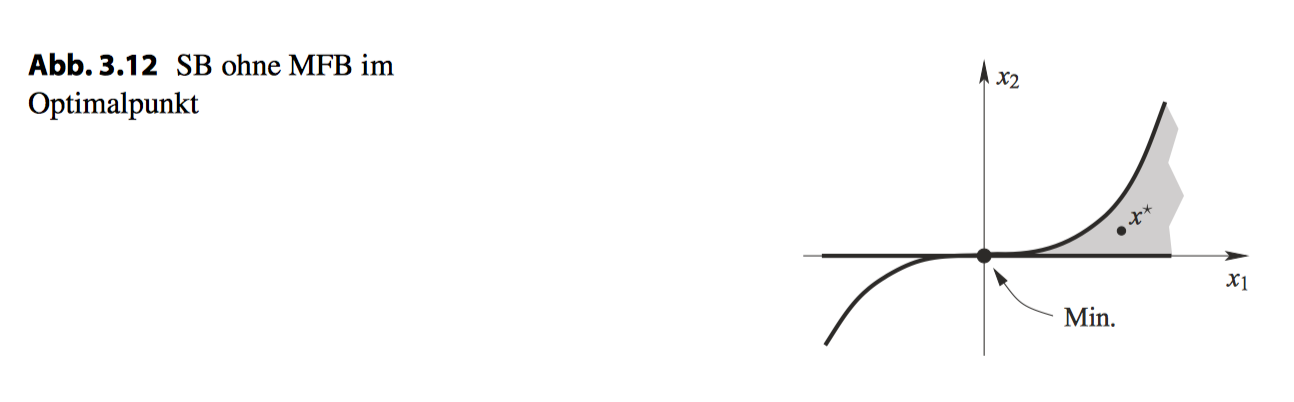
\includegraphics[scale=0.5]{ab312}
\end{center}

\begin{satz}
	Die Menge $M \subseteq \mathbb{R}^n$ sei konvex beschrieben, nichtleer, und die Funktionen $g_i \colon \mathbb{R}^n \rightarrow \mathbb{R}$, $i \in I$, seien zusätzlich stetig differenzierbar. Dann sind die folgenden Aussagen äquivalent:
	\begin{enumerate}[label=\alph*\upshape)]
		\item Die MFB gilt überall in $M$.
		\item Die MFB gilt irgendwo in $M$.
		\item $M$ erfüllt die SB.
	\end{enumerate}
\end{satz}

Dass die lokale Regularitätsbedingung MFB mit der globalen Regularitätsbedingung SB äquivalent sein kann, liegt an der Voraussetzung einer globalen Struktur an P, nämlich der Konvexität. ~\bigskip

Laut Korollar 2.1.41 sind im glatten konvexen unrestringierten Fall die kritischen Punkte mit den globalen Minimalpunkten identisch. Zu vermuten ist also, dass im restringierten Fall die KKT-Punkte den globalen Minimalpunkten entsprechen. Im Folgenden werden wir sehen, dass dies zumindest unter der SB richtig ist.

\begin{korollar}
	Das Problem $P$ sei konvex, und $M$ erfülle die $SB$. Dann ist jeder lokale Minimalpunkt von $P$ KKT-Punkt.
\end{korollar}

\begin{satz}
	Der Punkt $\overline{x}$ sei KKT-Punkt des konvexen Problems $P$. Dann ist $\overline{x}$ ein globaler Minimalpunkt von $P$.
\end{satz}

Im Gegensatz zur notwendigen Optimalitätsbedingung aus Korollar 3.2.76 benötigt die hinreichende Bedingung in Satz 3.2.77 keinerlei Regularitätsvoraussetzung. Insgesamt erhalten wir folgende \enquote{Charakterisierung} für globale Minimalpunkte konvexer Probleme P:

	$$ \overline{x} \text{ globaler Minimalpunkt } \xRightarrow[]{SB} \overline{x} \text{ KKT-Punkt } \Rightarrow \overline{x} \text{ globaler Minimalpunkt } $$

\section{Numerische Verfahren}

Dieser Abschnitt behandelt einige numerische Verfahren zur Lösung des Problems

$$ P: \quad \min_{x \in \mathbb{R}^n} f(x) ~\text{ s.t. } g_i(x) \leq 0, i \in I, h_j(x) = 0, j \in J, $$

mit hinreichend glatten Funktionen $f$, $g$ und $h$.

\subsection*{Straftermverfahren}

\begin{definition}[Straftermfunktion]
	Eine Funktion $\alpha \colon \mathbb{R}^n \rightarrow \mathbb{R}$ heißt Straftermfunktion für $M \subseteq \mathbb{R}^n$, falls folgende Bedingungen erfüllt sind:
	\begin{enumerate}[label=\alph*\upshape)]
		\item Für alle $x \in M$ gilt $\alpha(x) = 0$.
		\item Für alle $x \in Mc$ gilt $\alpha(x) > 0$.
	\end{enumerate}	
\end{definition}

Das Straftermverfahren bedient sich des Skalarisierungsansatzes zur Lösung des Mehrzielproblems, d. h., minimiert wird eine gewichtete Summe der beiden Zielfunktionen $f$ und $\alpha$. Aufgrund von Übung 1.3.1a genügt es dabei, nur eine der beiden Funktionen mit einem Gewicht zu versehen. Dies führt auf den Ansatz, $P$ durch ein unrestringiertes Problem mit Zielfunktion
$$ P(t): \min_{x \in \mathbb{R}^n} f(x) + t \cdot \alpha(x) $$

Die exakte Lösung von P würde man für jedes t mit der „idealen“ Straftermfunktion $\alpha(x) =  +\infty$ für alle $x \in M^c$ erhalten. Da dies nicht numerisch realisierbar ist, folgt mit
	$$ g_i^+(x) \coloneqq \max \{ 0, g_i(x) \}, ~ i \in I $$
Wegen der Definitheit von Normen betrachten wir mit einem $r \in \mathbb{N}$ der Term
$$ \alpha_r(x) \coloneqq \| (g_1^+(x), \dotsc, g_p^+(x), h_1(x), \dotsc, h_q(x)) \|_r^r $$
Diese verschwindet genau dann, wenn auch das Argument eintragsweise verschwindet.

\begin{uebung}
	Zeigen Sie mit Hilfe von Übung 2.1.12, dass die Funktionen $\varphi(a) = \max \{0, a\}$ und $abs(a) = |a|$ an jedem $a \in \mathbb{R}$ einseitig richtungsdifferenzierbar sind, und zwar mit für alle $d \in \mathbb{R}$ 
	$$ \varphi'(a, d) = \begin{cases}
		0, & \text{ falls } a < 0 \\
		\max \{ 0, d \}, & \text{ falls } a = 0 \\ d, & \text{ falls } a > 0
	\end{cases} $$
	$$ abs'(a, d) = \begin{cases}
		-d, & \text{ falls } a < 0 \\ |d|, & \text{ falls } a = 0 \\ d, & \text{ falls } a > 0
	\end{cases} $$
\end{uebung}

\begin{uebung}
	Für auf $\mathbb{R}^n$ stetig differenzierbare Funktionen $g$ und $h$ die einseitige Richtungsdifferenzierbarkeit der $\ell_1$-Straftermfunktion an jedem $x \in \mathbb{R}^n$ mit
	$$ \alpha_1'(x, d) = \sum_{i \in I_0(x)} \max \{ 0, \langle \nabla g_i(x), d \rangle \} + \sum_{i \in I_+(x)} \langle \nabla g_i(x), d \rangle - \sum_{j \in J_{-}(x)} \langle \nabla h_j(x), d \rangle $$
	$$  ~\hspace{3cm} + \sum_{j \in J_0(x)} |\langle \nabla h_j(x), d \rangle | + \sum_{j \in J_{+}(x)} \langle \nabla h_j(x), d \rangle $$
\end{uebung}

\begin{uebung}
	Die Funktion $\varphi^2(a) = (\max\{0, a\})^2$ ist an jedem $a \in \mathbb{R}$ stetig differenzierbar und für auf $\mathbb{R}^n$ stetig differenzierbare Funktionen $g$ und $h$ ist daher auch $\alpha_2$ auf ganz $\mathbb{R}^n$ stetig differenzierbar.
\end{uebung}

\begin{satz}
	Die Funktion $\alpha \colon \mathbb{R}^n \rightarrow \mathbb{R}$ sei eine stetige Straftermfunktion für $M$, $(t^k)$ sei eine monoton wachsende Folge mit $\lim_k t^k = +\infty$, und für alle $k \in \mathbb{N}$ sei $x^k$ ein globaler Minimalpunkt von $P(t^k)$. Dann ist jeder Häufungspunkt $x^*$ von $(x^k)$ ein globaler Minimalpunkt von $P$.
\end{satz}

\end{document}